\chapter{微分中值定理和Taylor展开式}
\section{微分中值定理}
\precis{Fermat引理,Rolle中值定理,Lagrange中值定理,Cauahy中值定理,微分Darboux定理,凸集,常微分方程初值问题解的唯一性}
\begin{quiza}
\woe 设一元实函数\(f\)在\([a,b]\)上连续, 在\((a,b)\)内可导, \(f(a)=f(b)=0\). 证明:
\begin{quizs}
\item 存在\(\xi\in(a,b)\)使得\(\xi^2f(\xi)++f'(\xi)=0\).
\begin{proof}
令\(F(x)=f(x)\cdot\exp\left(\frac{1}{3}x^3\right)\), 则\(F(0)=F(1)\), 由Rolle定理知\(\exists \xi\in(a,b)\)使得\(F'(\xi)=\exp\left(\frac{1}{3}\xi^3\right)\left(\xi^2f(\xi)+f'(\xi)\right)=0\), 结论得证.
\end{proof}
\item 存在\(\xi\in(a,b)\)使得\(f^2(\xi)\sin\xi++f'(\xi)=0\).
\begin{proof}
令\(F(x)=f(x)\cdot\exp\left(\int_a^x f(t)\sin t\dd t\right).\)仿(1)即可.
\end{proof}
\end{quizs}
\woe 设实函数\(f\)在\([a,b]\)上可导, \(f(a)=f(b)=0\). 证明: 存在\(\xi\in(a,b)\)使得\[f^3(\xi)+f'(\xi)=0.\]
\begin{proof}
令\(F(x)=f(x)\cdot\exp\left(\int_a^x f^2(t)\dd t\right)\), 则\(F(a)=F(b)=0\), 由Rolle定理知\(\exists \xi\in(a,b)\)使得\[F'(\xi)=\exp\left(\int_a^\xi f(t)\dd t\right)\left(f^3(\xi)+f'(\xi)\right)=0,\]从而得证.
\end{proof}
\woe 设实函数\(f\)在\([0,1]\)上连续, 在\((0,1)\)内二阶可导. 已知\(f(0)=f(1)=0,f\left(\frac{1}{2}\right)=\frac{1}{4}.\) 证明: 存在\(\xi\in(0,1)\), 使得\(f''(\xi)=-2\).
\begin{proof}
令\(F(x)=f(x)+x^2\), 则\(F(0)=0,F(1)=1,F\left(\frac{1}{2}\right)=\frac{1}{2}\), 则由Lagrange中值定理知\(\exists\xi_1\in \left(0,\frac{1}{2}\right),\xi_2\in\left(\frac{1}{2},1\right)\)使得\[F'(\xi_1)=\frac{F\left(1/2\right)-F(0)}{1/2-0}=1,\quad F'(\xi_2)=\frac{F(1)-F\left(1/2\right)}{1-1/2}=1,\]由Rolle定理知\(\exists\xi\in(\xi_1,\xi_2)\)使得\(F''(\xi)=f''(\xi)+2=0\). 得证.
\end{proof}
\woe 设实函数\(f\)在\([0,1]\)上有二阶导数, 且\[f(0)=1,\quad f(1)=3\ee,\quad f'(1)=5\ee.\]证明或证伪: 存在\(\xi\in(0,1)\)使得\[f''(\xi)-2f'(\xi)+f(\xi)=0.\]
\begin{proof}
令\(F(x)=\ee^{-x}f(x).\) 则\(F(0)=1,F(1)=3\), 由Lagrange中值定理知\(\exists \xi_1\)使得\[F'(\xi_1)=\frac{F(1)-F(0)}{1-0}=2,\]而易见\(F'(1)=2\), 从由Rolle定理\(\exists \xi\in(\xi_1,1)\)使得\(F''(\xi)=\ee^{-\xi}\left(f''(\xi)-2f'(\xi)+f(\xi)\right)=0\).
\end{proof}
\woe 设一元实函数\(f\)在\([1,2]\)上有二阶导数, 且\(f(2)=0\). 令\(F(x)=(x-1)^2f(x)\), 证明: 存在\(\xi\in(1,2)\)使得\(F''(\xi)=0.\)
\begin{proof}
易见\(F(1)=F(2)=0\), 由Rolle定理知\(\exists \xi_1\in(a,b)\)使得\(F'(\xi_1)=0\), 易见\(F'(1)=0\), 再次使用Rolle定理知\(\xi\in(\xi_1,1)\)使得\(F''(\xi)=0\).
\end{proof}
\woe 设\(\delta>0\). 在\((-\delta,\delta)\)内, 一元实函数\(f\)可微, 且满足\[f(x+y)=\frac{f(x)+f(y)}{1-f(x)f(y)},\quad\forall x,y,x+y\in(-\delta,\delta).\]试求\(f\).
\begin{solution}
易见\(f(0)=0\), 方程两侧对\(y\)求导得到\[f'(x+y)=\frac{f'(y)\left(1-f(x)f(y)\right)+f(x)f'(y)\left(f(x)+f(y)\right)}{\left(1-f(x)f(y)\right)^2},\]记\(a=f'(0)\), 同时令\(y=0\)得到\[f'(x)=a+af^2(x),\]容易解得\(f(x)=\tan ax.\)
\end{solution}
\woe 设\(a_1=2,a_2=3,a_{n+2}=a_{n+1}+\frac{1}{\ln a_n}(n\geqslant 1)\). 证明: \(\lim_{n\rightarrow+\infty}\frac{a_n\ln a_n}{n}\)存在并求其值.
\begin{solution}
易见\(\{a_n\}\)单增且无界. 设可微函数\(f(x)\)满足\(f(n)=a_n\), 且\(f(x)\)单调递增. 同时设\(F(x)=f(x)\ln f(x)\). 对于原极限, 由Stolz定理与Lagrange中值定理可得\[\lim_{n\rightarrow+\infty}\frac{a_n\ln a_n}{n}=\lim_{n\rightarrow+\infty}a_{n+1}\ln a_{n+1}-a_n\ln a_n=\lim_{n\rightarrow+\infty}F(n+1)-F(n)=\lim_{n\rightarrow+\infty}F'(\xi_n),\]其中\(\xi_n\in(n,n+1)\), 而\(F'(x)=f'(x)\left(\ln f(x)+1\right)\), 结合\(f(x)\)单调性, 有\[f'(\xi_n)\left(\ln a_n+1\right)\leqslant f'(\xi_n)\left(\ln\xi_n+1\right)\leqslant f'(\xi_n)\left(\ln a_{n+1}+1\right).\]
\(\lim_{n\rightarrow+\infty}\frac{a_n\ln a_n}{n}=1.\)
\end{solution}
\woe 设\(\psi\)是\((0,+\infty)\)上局部有界的实值函数, 满足\[\psi(xy)=\psi(x)+\psi(y),\qquad\forall x,y\in(0,+\infty).\]试证明:
\begin{quizs}
\item \(\psi\)在\((0,+\infty)\)上某一点连续, 进而在\((0,+\infty)\)每一点连续.
\item 对任何\(x>0\)以及有理数\(q\), \(\psi(x^q)=q\psi(x).\)
\item 对任何\(x>0\)以及实数\(y\), \(\psi(x^y)=y\psi(x).\)
 
特别的, 对任何\(x>0\)成立\(\psi(x)=\psi(\ee)\ln x.\)
\end{quizs}
\woe 若对任何\(x,y\in\mathbb{R},\mathbb{R}\)上不恒为零的一元实函数\(f\)满足\(f(x+y)=f(x)f(y)\). 进一步, \(f\)在\(\mathbb{R}\)上局部有界, 证明: 存在常数\(a\)使得\[f(x)=a^x,\qquad\forall x\in\mathbb{R}.\]
\woe 举例说明中值定理对于复值函数不成立.
\woe 设\(f,g\in C[a,b],g\)严格单调. 证明: 存在\([a_1,b_1]\subset [a,b]\)使得\(b_1-a_1=\frac{b-a}{2}\), 且\[\frac{f(b_1)-f(a_1)}{g(b_1)-g(a_1)}=\frac{f(b)-f(a)}{g(b)-g(a)}.\]
\begin{proof}
记\(m=\frac{a+b}{2},c=\frac{b-a}{2}\), 设\[F(x)=\frac{f(x+c)-f(x)}{g(x+c)-g(x)}-\frac{f(b)-f(a)}{g(b)-g(a)},\quad x\in[a,m],\]注意到\[\frac{f(m)-f(a)}{g(m)-g(a)}\cdot\frac{g(m)-g(a)}{g(b)-g(a)}+\frac{f(b)-f(m)}{g(b)-g(m)}\cdot\frac{g(b)-g(m)}{g(b)-g(a)}=\frac{f(b)-f(a)}{g(b)-g(a)},\]并且\(\frac{g(m)-g(a)}{g(b)-g(a)}+\frac{g(b)-g(m)}{g(b)-g(a)}=1\), 结合题设可知\(F(a)\)与\(F(c)\)异号, 从而有结论得证.
\end{proof}
\end{quiza}
\begin{quizb}
\woe 若对任何\(x,y\in\mathbb{R},\mathbb{R}\)上的一元复值函数\(f\)满足\(f(x+y)=f(x)f(y)\). 进一步, \(f\)在\(\mathbb{R}\)上局部有界. 试问, \(f\)的解具有什么形式?
\woe 在上一题中, 假设\(f\)的取值为\(n\)阶方阵, 结论又如何?
\woe 设\(f\)在\((a,b)\)内连续且右导数为\(f'_+(x)=x\arctan x\). 证明: \(f\)在\((a,b)\)内可导.
\woe 设实函数\(f\)在\(\left[0,+\infty\right)\)上有二阶的连续导数, 满足\(f(0)=f'(0)=0\)以及\(f''(x)+3f'(x)+2f(x)\geqslant 0\). 证明: \(f(x)\geqslant 0\left(\forall x\in \left[0,+\infty\right)\right)\).
\woe 设实函数\(f\)在区间\([-1,1]\)上连续, 在\((-1,1)\)内三阶可导. 证明: \(\xi\in(-1,1)\)使得\(f'''(\xi)=3\left(f(1)-f(-1)-2f'(0)\right)\).
\begin{proof}
令\[\begin{split}
F(x)=&f(x)-\left(\frac{f(1)-f(-1)-2f'(0)}{2}\right)x^3+\left(f(0)-\frac{f(-1)+f(1)}{2}\right)x^2-f'(0)x
\end{split}\]于是有\[F(-1)=F(0)=F(1)=f(0),\]由Rolle定理可知\(\exists \xi_1\in(-1,0),\exists \xi_2\in(0,1)\)使得\(F'(\xi_1)=F'(\xi_2)=0\), 又有\(F'(0)=0\),再次使用Rolle定理, 即\(\exists \xi_3\in(\xi_1,0)\)与\(\xi_4\in(0,\xi_2)\)使得\(F''(\xi_3)=F''(\xi_4)=0\), 依Rolle定理\(\exists \xi\in(\xi_3,\xi_4)\)使得\(F'''(\xi)=0\). 结论得证.
\end{proof}
\woe 设实函数\(f\)为\(\mathbb{R}\)上的有界可微函数, 且对任何\(x\)均有\(|f'(x)|<1.\) 证明: 存在\(M<1\)使得对任何\(x\in\mathbb{R}\)成立\(|f(x)-f(0)|\leqslant M|x|\).

进一步, 是否存在常数\(K<1\), 使得对任何\(x,y\in\mathbb{R}\), 均有\(|f(x)-f(y)|<K|x-y|\)?
\begin{proof}
由Lagrange中值定理, 有\[\left|\frac{f(x)-f(0)}{x-0}\right|=|f'(\xi)|<M<1,\quad \xi\text{介于\(0\)与\(x\)之间},\]由此知\(|f(x)-f(0)|<M|x|\). 同理可知后者部分结论也成立.
\end{proof}
\woe 设实函数\(f\)是\(\mathbb{R}\)上的连续可导函数, 且\(\forall x\in\mathbb{R}, f'(x)>f\left(f(x)\right)\). 证明: \(\forall x\geqslant 0,f\left(f\left(f(x)\right)\right)\leqslant 0\).
\begin{proof}
我们先证明\(\lim_{x\rightarrow+\infty}f(x)\ne +\infty\). 若\(\lim_{x\rightarrow+\infty}f(x)= +\infty\), 则\(\exists X_1,\forall x>X_1\)有\(f(x)>2\), 也有\(X_2\)使得\(\forall x>X_2\)有\(f(x)>X_1\), 这样就有\[f'(x)>f\left(f(x)\right)>f(X_1)>2,\quad \forall x>X_2,\]因此有\(X_3\)使\(x>X_3-1\)时有\(f(x)>x\)成立, 也即\(f'(x)>f\left(f(x)\right)>f(x)\), 有\(\frac{f'(x)}{f(x)}>1\), 即有\[\int_{X_3}^{x}\frac{f'(x)}{f(x)}\dd x=\ln f(x)-\ln f(X_3)>t-X_3\Rightarrow f(x)>f(X_3)\ee^{x-X_3}>X_3\ee^{x-X_3},\]于是有\[f'(x)>f\left(f(x)\right)>X_3\ee^{f(x)-X_3}\Rightarrow f'(x)\ee^{-f(x)}>X_3\ee^{-X_3},\]由此得出\[\int_{X_3}^{x}f'(x)\ee^{-f(x)}\dd x>\int_{X_3}^{x}X_3\ee^{-X_3}\Rightarrow \ee^{-f(X_3)}-\ee^{-f(x)}>(x-X_3)X_3\ee^{-X_3},\]矛盾, 从而\(\lim_{x\rightarrow+\infty}f(x)\ne +\infty\).

由此可得存在一些\(x>0\)使得\(f(x)<x\), 下面我们证明, 不可能有\(x_0>0\)使得\(f(x_0)=x_0\), 从而\(\forall x>0\)都有\(f(x)<x\). 如若这样的\(x_0\)存在, 我们先证明\(\forall x\geqslant x_0\), 有\(f(x)\geqslant x_0\), 事实上这也是不可能的, 因为此时有\[f'(x)>f\left(f(x)\right)\geqslant f(x_0)=x_0>0,\quad\forall x\geqslant x_0,\]这与\(\lim_{x\rightarrow+\infty}f(x)\ne +\infty\)矛盾. 下面我们证明前述结论, 事实上如果存在\(x\geqslant x_0\)而\(f(x)<x_0\), 我们考虑\(T=\inf\{x\geqslant x_0\big| f(x)<x_0\}\), 则由\(f\)的连续性可知\(f(T)=x_0\), 于是\[f'(T)>f\left(f(T)\right)=f(x_0)=x_0>0,\]这意味着存在\(\delta>0\)使得\(x\in(T-\delta,T)\)时有\(f(x)<f(T)=x_0\), 这与\(T\)的定义矛盾.

下面我们证明: 若\(f(x_1)>0\)且\(f(x_2)\geqslant x_1\), 那么\(\forall x>x_2\)都有\(f(x)>x_1\). 特别的, 如果\(x_1\leqslant 0\)且\(f(x_1)> 0\), 那么\(\forall x>x_1\)有\(f(x)>x_1\).

若存在\(x>x_2\)但\(f(x)\leqslant x_1\), 我们考虑\(S=\inf\{x>x_2\big|f(x)\leqslant x_1\}\), 由\(f\)的连续性可知\(f(S)=x_1\), 类似于前面的证明, 我们有\[f'(S)>f\left(f(S)\right)=f(x_1)>0,\]如果\(S>x_2\), 则有\(\delta_1>0\)使得\(x\in(S-\delta_1,S)\)时有\(f(x)<f(S)=x_1\)与\(S\)的定义矛盾, 如果\(S=x_2\), 则有\(\delta_2>0\)使得\(x\in(S,S+\delta_2)\)有\(f(x)>s_1\), 仍矛盾. 而后者只需考虑\(x_1=x_2\).


\end{proof}


\end{quizb}
\section{L'H\^{o}pital法则}
\precis{L'H\^{o}pital法则及其推广,极限计算的化简---“去核”和"去皮"}
\begin{quiza}
\woe 设\(x_0\in(0,\pi),x_{n+1}=\sin x_n(n\geqslant 0).\) 计算\(\lim_{n\rightarrow+\infty}\sqrt{n}\sin x_n\).
\begin{solution}
易见\(\{x_n\}\)大于零单调递减有下界, 取极限得\(\lim_{n\rightarrow\infty}x_n=0\), 而\[\begin{split}
\lim_{n\rightarrow\infty}\frac{1}{n\sin^2 x_n}&\xlongequal{\text{Stolz}}\lim_{n\rightarrow\infty}\frac{\sin^2x_n-\sin^2x_{n+1}}{\sin^2x_n\sin^2x_{n+1}}=\lim_{n\rightarrow\infty}\frac{x_{n+1}^2-\sin^2x_{n+1}}{x_{n+1}^2\sin^2x_{n+1}}\\&=\lim_{x\rightarrow 0}\frac{(x-\sin x)(x+\sin x)}{x^2\sin^2x}=\lim_{x\rightarrow 0}\frac{1/6\cdot x^3\cdot 2x}{x^4}=\frac{1}{3}.
\end{split}\]从而\(\lim_{n\rightarrow+\infty}\sqrt{n}\sin x_n=\sqrt{3}\).
\end{solution}
\woe 计算\(\lim_{x\rightarrow 0}\left(\frac{\arcsin x}{x}\right)^{1/x^2}\).
\begin{solution}
由于\[\lim_{x\rightarrow 0}\frac{\ln\left(\dfrac{\arcsin x}{x}\right)}{x^2}=\lim_{x\rightarrow 0}\frac{\arcsin x-x}{x^3}=\frac{1}{6}.\]从而\(\lim_{x\rightarrow 0}\left(\frac{\arcsin x}{x}\right)^{1/x^2}=\exp\left(\frac{1}{6}\right)\).
\end{solution}
\woe 计算\(\lim_{x\rightarrow+\infty}\left(\left(x^3-x^2+\frac{x}{2}\right)\ee^{1/x}-\sqrt{x^6+x}\right)\).
\begin{solution}
令\(t=\frac{1}{x}\), 则原极限变为\[\lim_{t\rightarrow0^+}\frac{\ee^t\left(1-t+\dfrac{1}{2}t^2\right)-\sqrt{1+t^5}}{t^3}\xlongequal{\text{L'H\^{o}pital}}\lim_{t\rightarrow 0^+}\frac{\dfrac{1}{2}t^2\ee^t-\dfrac{5t^4}{2\sqrt{1+t^5}}}{3t^2}=\frac{1}{6}.\qedhere\]
\end{solution}
\woe 计算:
\begin{quizs}
\item \(\lim_{x\rightarrow 0}\frac{\arctan(\sin x)-\arctan(\ln (1+x))}{x^2}\).
\begin{solution}
注意到\(\lim_{x\rightarrow 0}\frac{\sin x-\ln(1+x)}{x^2}\xlongequal{\text{L'H\^{o}pital}}\frac{1}{2}\), 于是有\[\begin{split}
&\lim_{x\rightarrow 0}\frac{\arctan(\sin x)-\arctan(\ln (1+x))}{x^2}\\=&\lim_{x\rightarrow 0}\frac{\arctan(\sin x)-\arctan(\ln (1+x))}{\sin x-\ln(1+x)}\cdot\frac{\sin x-\ln(1+x)}{x^2}\\=&\frac{1}{2}\lim_{x\rightarrow 0}\left(\arctan x\right)'=\frac{1}{2}.\qedhere
\end{split}\]
\end{solution}
\item \(\lim_{x\rightarrow 0}\frac{(1+\tan x)^{3/2}-(1+x)^{3/2}}{x^3}.\)
\begin{solution}
注意到\(\lim_{x\rightarrow 0}\frac{\tan x-x}{x^3}\xlongequal{\text{L'H\^{o}pital}}=\frac{1}{3}\), 于是有\[\begin{split}
&\lim_{x\rightarrow 0}\frac{(1+\tan x)^{3/2}-(1+x)^{3/2}}{x^3}=\lim_{x\rightarrow 0}\frac{(1+\tan x)^{3/2}-(1+x)^{3/2}}{\tan x-x}\cdot\frac{\tan x-x}{x^3}\\=&\frac{1}{3}\lim_{x\rightarrow 0}\left((1+x)^{3/2}\right)'=\frac{1}{2}.\qedhere
\end{split}\]
\end{solution}
\item \(\lim_{x\rightarrow 0}\left(\frac{1}{\ln (x+\sqrt{1+x^2})}-\frac{1}{\ln(1+x)}\right).\)
\begin{solution}
记\(F(x)=\ln(1+x),\varphi(x)=x,\psi(x)=x+\sqrt{1+x^2}-1\), 注意到\[\lim_{x\rightarrow 0}F'(x)=1,\quad\lim_{x\rightarrow 0}\frac{\varphi(x)}{x}=\lim_{x\rightarrow 0}\frac{\psi(x)}{x}=1,\]以及\begin{gather*}
\lim_{x\rightarrow 0}\frac{\varphi(x)-\psi(x)}{x^2}=\lim_{x\rightarrow 0}\frac{1-\sqrt{1+x^2}}{x^2}\xlongequal{\text{L'H\^{o}pital}}-\frac{1}{2}\\
\lim_{x\rightarrow 0}\frac{\varphi(x)\psi(x)}{x^2}=\lim_{x\rightarrow 0}\frac{\varphi(x)}{x}\cdot\lim_{x\rightarrow 0}\frac{\psi(x)}{x}=1.
\end{gather*}
从而\[\begin{split}
&\lim_{x\rightarrow 0}\left(\frac{1}{\ln (x+\sqrt{1+x^2})}-\frac{1}{\ln(1+x)}\right)=\lim_{x\rightarrow 0}\frac{\ln(1+x)-\ln\left(x+\sqrt{1+x^2}\right)}{\ln (x+\sqrt{1+x^2})\cdot\ln(1+x)}\\
=&\lim_{x\rightarrow 0}\frac{\ln(1+x)-\ln\left(x+\sqrt{1+x^2}\right)}{x^2}=-\frac{1}{2}.\qedhere
\end{split}\]
\end{solution}
\item \(\lim_{x\rightarrow 0}\frac{\left(1+\frac{x}{x+1}\right)^{(1+x)/x}-\left(1+\tan x\right)^{1/\tan x}}{x^2}\).
\begin{solution}
设\(F(x)=\left(1+x\right)^{1/x}\), 注意到\[\lim_{x\rightarrow 0}\frac{\frac{x}{x+1}-\tan x}{x^2}=\lim_{x\rightarrow0}\frac{x-(x+1)\tan x}{x^2}\xlongequal{\text{L'H\^{o}pital}}-1,\]以及\[\lim_{x\rightarrow 0}F'(x)=\ee\lim_{x\rightarrow 0}\frac{x-(1+x)\ln(1+x)}{x^2}\xlongequal{\text{L'H\^{o}pital}}-\frac{\ee}{2}.\]于是\[\begin{split}
&\lim_{x\rightarrow 0}\frac{\left(1+\frac{x}{x+1}\right)^{(1+x)/x}-\left(1+\tan x\right)^{1/\tan x}}{x^2}\\=&\lim_{x\rightarrow 0}\frac{\left(1+\frac{x}{x+1}\right)^{(1+x)/x}-\left(1+\tan x\right)^{1/\tan x}}{\frac{x}{x+1}-\tan x}\cdot\frac{\frac{x}{x+1}-\tan x}{x^2}=\frac{\ee}{2}.\qedhere
\end{split}\]
\end{solution}
\end{quizs}
\woe 设\(f\)在\([a,b]\)上两阶可导, 且满足\(|f''(x)|\leqslant M|f(x)|,f(a)=f'(a)=0\), 其中\(M\)是一个常数, 证明\(f(x)\equiv 0\).
\begin{proof}
97页

反证法. 若\(\exists x_0\in(a,b]\)使得\(f(x_0)\ne 0\), 不妨设\(f(x_0)>0\), 记\[c=\sup\{x\in[a,x_0]\big|f(x)\leqslant 0\},\]则\(c\)适定, 且\(c\in\left[a,x_0\right),f(c)=0\),\[f(x)>0,\qquad\forall x\in(c,x_0).\]在\((c,x_0)\)内, 有\[\frac{f'(x)}{f(x)}\leqslant M,\]即\[\left(\ln f(x)\right)'\leqslant M,\forall x\in(c,x_0),\]所以由中值定理可得\[\frac{\ln f(x_0)-\ln f(x)}{x_0-c}\leqslant M,\quad\forall x\in(c,x_0).\]在上式中令\(x\rightarrow c^+\), 并注意到\(f(c)=0\)得到\(+\infty\leqslant M\). 矛盾, 所以\(f(x)\equiv 0\).
\end{proof}
\woe 设\(f\)在\(\left[0,+\infty\right)\)可导, 且\(f'(x)\)在\(\left(0,+\infty\right)\)上一致连续, \(\lim_{x\rightarrow+\infty}f(x)\)存在. 证明\(\lim_{x\rightarrow+\infty}f'(x)=0.\)
\begin{proof}

\end{proof}
\woe 设\(f\)在\(\mathbb{R}\)上连续可微, 且\(f(x+1)-f(x)=f'(x)(\forall x\in\mathbb{R})\), \(\lim_{x\rightarrow+\infty}f'(x)=c.\)证明\(f'(x)\equiv c\).
\begin{proof}
反证法. 设有\(\xi_0\)使得\(f'(\xi_0)\ne c\), 则\[f(\xi_0+1)-f(\xi_0)=f'(\xi_0),\] 由Lagrange中值定理可知\(\exists \xi_1\in(\xi_0,\xi_0+1)\)使得\[f'(\xi_0)=f(\xi_0+1)-f(\xi_0)=f'(\xi_1),\] 则\(f(\xi_1+1)-f(\xi_1)=f'(\xi_1)\)又由Lagrange中值定理知\(\exists \xi_2\in(\xi_1,\xi_1+1)\)使得\[f'(\xi_0)=f(\xi_1+1)-f(\xi_1)=f'(\xi_2),\]重复这个操作得到\(\{\xi_n\}\)使得\(f'(\xi_n)=f'(\xi_0)(n=0,1,2\cdots)\), 设集合\(E\)为全体导数值等于\(f'(\xi_0)\)的坐标全体, 即\[E=\{\xi\big|f'(\xi)=f'(\xi_0)\},\]由上面的信息可见\(E\)为无限集。

若\(E\)无界, 则与题设\(\lim_{x\rightarrow+\infty}f'(x)=c.\)矛盾. 下证\(E\)必无界. 

事实上, 若\(E\)有界, 则必有上确界, 记\(\sup_{\xi\in E}\xi =M\), 从\(E\)中选取一子列\(\{\xi'_n\}\)使其收敛于\(M\), 结合\(f(x)\)的连续性有\[f'(\xi_0)=\lim_{n\rightarrow\infty}\left[f(\xi'_n+1)-f(\xi'_n)\right]=f(M+1)-f(M),\]由Lagrange中值定理可知\(\exists \xi'\in(M,M+1)\)使得\(f'(\xi')=f'(\xi_0)\), 即\(\xi'\in E\)并且\(\xi'>M\), 矛盾. 进而\(E\)无界.
\end{proof}
\end{quiza}
\begin{quizb}
\woe 设\(x\in(0,1),p>0\), 试考察级数\[\left(\sin x\right)^p-\left(\sin\left(\sin x\right)\right)^p+\left(\sin\left(\sin\left(\sin x\right)\right)\right)^p-\left(\sin\left(\sin\left(\sin\left(\sin x\right)\right)\right)\right)^p+\cdots\]的收敛性(含绝对收敛性).
\begin{solution}
记\(a_0=x\), \(a_{n+1}=\sin a_n(n\geqslant 1)\), 于是原级数即为\(\sum_{n=1}^{\infty}(-1)^{n+1}a_n\), 参考6.2\(\boldsymbol{\mathcal{A}}\)可知\(\{a_n^p\}\)单调递减趋于零, 由Leibniz判别法可知原级数收敛. 

并且由\(\lim_{n\rightarrow+\infty}\sqrt{n}\sin a_n=\sqrt{3}\)可知\(a_n\sim\sqrt{\frac{3}{n}}\), 即\(a_n^p\sim\left(\frac{3}{n}\right)^{p/2}\), 从而\(p>2\)时原级数绝对收敛.
\end{solution}
\woe 设\(n\geqslant 1,P\)为\(n\)阶实系数多项式, 则对于\(\mathbb{R}\)上任何\(n\)次可导的实函数\(f\), \(\lim_{x\rightarrow +\infty}P(\DD)f(x)=0\)均蕴涵\(\lim_{x\rightarrow+\infty}f(x)=0\)的充要条件是\(P\)的所有零点都有负实部.
\begin{proof}
	必要性.
    
    充分性.
\end{proof}
\woe 设\(f\)在\(\left[1,+\infty\right)\)上连续, 在\(\left(1,+\infty\right)\)上可导, 且\(\ee^{x^2}f'(x)\)在\(\left(1,+\infty\right)\)上有界, 则在什么条件下可得\(x\ee^{x^2}f(x)\)在\(\left[1,+\infty\right)\)上有界?
\begin{solution}
	
\end{solution}
\woe 设实函数\(f\)在\(\mathbb{R}\)上有界, 可导且\(|f'(x)|<1(\forall x\in\mathbb{R})\), 又设\(x_0\in\mathbb{R},x_{n+1}=f(x_n)(n\geqslant 0)\), 证明\(\{x_n\}\)收敛.
\begin{proof}
设\(\max\{\left|f(x)\right|,|x_0|\}\leqslant M\). 考虑\(F(x)=x-f(x)\), 由于\(F(-M)=-M-f(-M)\leqslant 0\), 而\(F(M)=M-f(M)\geqslant 0\), 从而有\(x^*\in[-M,M]\)使得\(F(x^*)=0\). 下面说明, 这样的\(x^*\)是唯一的, 事实上由于\(|f'(x)|<1\), 由Lagrange中值定理, 对任意\(x<y\), 存在\(\xi\in(x,y)\)使得\[\left|f(x)-f(y)\right|=|f'(\xi)||x-y|<|x-y|,\]若还有\(x'\ne x^*\)使得\(F(x')=0\), 则有\(\left|f(x^*)-f(x')\right|=|x^*-x'|\)矛盾.

再证\(\{x_n\}\)收敛到\(x^*\), 由于\[\left|x_{n+1}-x^*\right|=\left|f(x_n)-f(x^*)\right|<\left|x_n-x^*\right|,\]从而\(\{|x_n-x^*|\}\)单调递减, 设其极限为\(A\), 则\(\{x_n\}\)必存在子列收敛到\(x^*\pm A\). 不妨设\(\{x_n\}\)本身收敛到\(x^*+A\), 则\(x_{n+1}=f(x_n)\)收敛到\(f(x^*+A)\), 也即\(x^*+A=f(x^*+A)\), 则\(F(x^*+A)=0\), 由上述知\(A\)只能为0. 从而\(\{x_n\}\)收敛.
\end{proof}
\woe 设实函数\(f\)在\(\mathbb{R}\)上可导且\(|f'(x)|<1(\forall x\in\mathbb{R})\), 又设\(x_0\in\mathbb{R},x_{n+1}=f(x_n)(n\geqslant 0)\), 证明\(\{x_n\}\)收敛或举例说明\(\{x_n\}\)可能发散.
\begin{solution}
\(\{x_n\}\)可能发散. 设\[f(x)=\begin{cases}
x+\frac{1}{x},&x\geqslant 1,\\
2,&-1<x<1,\\
-x-\frac{1}{x},&x\leqslant -1
\end{cases}\]
取\(x_0=1\)易见\(\{x_n\}\)发散.
\end{solution}
\woe 设\(\boldsymbol{F}:\mathbb{R}^n\rightarrow\mathbb{R}^n\)是可微的有界函数, \(\left\| \boldsymbol{F_x}(\boldsymbol{x})\right\|<1(\forall\boldsymbol{x}\in\mathbb{R}^n)\), 又设\(\boldsymbol{x}_0\in\mathbb{R}^n,\boldsymbol{x}_{k+1}=\boldsymbol{F}(\boldsymbol{x}_k)(k\geqslant 0)\), 证明\(\{\boldsymbol{x}_k\}\)收敛.
\begin{proof}
设\(\max\{\left\|\boldsymbol{F}(\boldsymbol{x})\right\|,\left\|\boldsymbol{x}\right\|\}\leqslant M\). 考虑\(\boldsymbol{G}(\boldsymbol{x})=\boldsymbol{x}-\boldsymbol{F}(\boldsymbol{x})\)在\([-M,M]^n\)上的结果. 对于\(\boldsymbol{x}\in\bbr^n\), 我们称\(\boldsymbol{x}\leqslant \boldsymbol{0}\)为\(\boldsymbol{x}\)的所有分量小于等于\(0\); \(\boldsymbol{x}\geqslant \boldsymbol{0}\)为\(\boldsymbol{x}\)的所有分量大于等于\(0\). 记\(\boldsymbol{M}\)为所有分量均为\(M\)的向量, 则\(\boldsymbol{G}(-\boldsymbol{M})\leqslant 0\)而\(\boldsymbol{G}(\boldsymbol{M})\geqslant 0\), 由于\([-M,M]^n\)道路连通并且\(\boldsymbol{G}\)连续, 从而有\(\boldsymbol{x^*}\in[-M,M]^n\)使得\(\boldsymbol{G}(\boldsymbol{x^*})=\boldsymbol{0}\).

下面说明这样的\(\boldsymbol{x^*}\)是唯一的, 事实上由于\(\left\| \boldsymbol{F_x}(\boldsymbol{x})\right\|<1\), 由中值定理, 对任意\(\boldsymbol{x},\boldsymbol{y}\), 存在\(\boldsymbol{\xi}\)使得\[\left\|\boldsymbol{F}(\boldsymbol{x})-\boldsymbol{F}(\boldsymbol{y})\right\|=\left\| \boldsymbol{F_x}(\boldsymbol{x})\right\|\left\|\boldsymbol{x}-\boldsymbol{y}\right\|<\left\|\boldsymbol{x}-\boldsymbol{y}\right\|,\]
若还有\(\boldsymbol{x'}\ne\boldsymbol{x^*}\)使得\(\boldsymbol{G}(\boldsymbol{x'})=\boldsymbol{0}\), 则有\(\left\|\boldsymbol{F}(\boldsymbol{x^*})-\boldsymbol{F}(\boldsymbol{x'})\right\|=\left\|\boldsymbol{x^*}-\boldsymbol{x*}\right\|\)矛盾. 其余部分参考第4题.
\end{proof}
\end{quizb}
\section{凸函数}
\precis{凸(凹)函数,Jensen不等式,割线斜率与凸性,凸性与连续性,中点凸(凹)函数,凸函数与一阶导数,支撑线(面),凸性与二阶导数,Hesse矩阵,对偶数,Young不等式,离散H\''{o}lder不等式,离散Minkowski不等式,幂平均不等式,调和平均}
\begin{definition}{}{C61}
设\(E\subseteq\mathbb{R}^n\)为凸集, 称\(f:E\rightarrow\mathbb{R}\)为\(E\)上的\textbf{凸函数}, 如果对于任何\(\alpha\in(0,1)\)以及\(\boldsymbol{x,y}\in E\), 成立\[f(\alpha\boldsymbol{x}+(1-\alpha)\boldsymbol{y})\leqslant\alpha f(\boldsymbol{x})+(1-\alpha)f(\boldsymbol{y}).\]若当\(\boldsymbol{x}\ne\boldsymbol{y}\)时上式中的严格不等式成立, 则称\(f\)为\textbf{严格凸函数}. 称\(f\)为\textbf{(严格)凹函数}如果\(-f\)是(严格)凸函数.
\end{definition}
\begin{definition}{}{C62}
    设\(E\subseteq\mathbb{R}^n\)为凸集, 称\(f:E\rightarrow\mathbb{R}\)为\(E\)上的\textbf{凸函数}, 如果对于任何\(m\geqslant 2,\boldsymbol{x}_1,\boldsymbol{x}_2,\cdots,\boldsymbol{x}_m\in E\)以及满足\(\alpha_1+\alpha_2+\cdots+\alpha_m=1\)的\(\alpha_1,\alpha_2,\cdots,\alpha_m\geqslant 0\) 成立\[f\left(\sum_{k=1}^{m}\alpha_k\boldsymbol{x}_k\right)\leqslant\sum_{k=1}^{m}\alpha_kf\left(\boldsymbol{x}_k\right).\]
\end{definition}
\begin{theorem}{}{C63}
设\(f\)为区间\((a,b)\)内的实连续函数. 则有\begin{compactenum}[(i)]
\item \(f\)(严格)凸当且仅当\(f'_+\)在\((a,b)\)内存在且(严格)单增.
\item \(f\)凸当且仅当\(f'_+\)在\((a,b)\)内存在, 且对任何\(x_0\in (a,b)\), 成立\[f(x)\geqslant f(x_0)+f_+'(x_0)(x-x_0),\quad\forall x\in (a,b).\]

而\(f\)严格凸当且仅当\(f'_+\)在\((a,b)\)内存在, 且对任何\(x_0\in (a,b)\)以及\(x\ne x_0\), 上式中严格不等式成立.
\item \(f\)(严格)凸当且仅当\(f'_-\)在\((a,b)\)内存在, 且\(f'_-\)(严格)单增.
\item \(f\)凸当且仅当\(f'_-\)在\((a,b)\)内存在, 且对任何\(x_0\in (a,b)\), 成立\[f(x)\geqslant f(x_0)+f_-'(x_0)(x-x_0),\quad\forall x\in (a,b).\]

而\(f\)严格凸当且仅当\(f'_-\)在\((a,b)\)内存在, 且对任何\(x_0\in (a,b)\)以及\(x\ne x_0\), 上式中严格不等式成立.
\item 若\(f\)可导, 则\(f\)(严格)凸当且仅当\(f'\)(严格)单增.
\item 若\(f\)可导, 则\(f\)凸当且仅当\textbf{曲线在切线之上}, 即对任何\(x_0\in (a,b)\), 成立\[f(x)\geqslant f(x_0)+f_-'(x_0)(x-x_0),\quad\forall x\in (a,b).\]而\(f\)严格凸当且仅当对任何\(x_0\in (a,b)\)以及\(x\ne x_0\), 上式中严格不等式成立.
\end{compactenum}
\end{theorem}
\begin{theorem}{}{C64}
设\(f\)为区间\((a,b)\)内二阶可导函数, 则\(f\)为凸函数当且仅当\(f''\)非负, 进一步, 若\(f''\)恒正, 则\(f\)严格凸.
\end{theorem}
\begin{quiza}
\woe 设\(E\subseteq\mathbb{R}^n\)为凸集. 证明\(f:\, E\rightarrow\mathbb{R}\)为凸函数当且仅当集合\(\{(\boldsymbol{x},y)|y\geqslant f(\boldsymbol{x},\boldsymbol{x}\in E)\}\)为凸集.
\begin{proof}

\end{proof}
\woe 证明: 凸函数的定义 \reff{Def:C61} 与定义 \reff{Def:C62} 等价.
\begin{proof}
content...
\end{proof}
\woe 设区间\(I\)上的实函数\(f\)在某一点\(x_0\in I\)的附近有界, 且\(f\)为\(I\)上的中点凸函数. 尝试按以下步骤证明\(f\)为\(I\)上的凸函数:\begin{quizs}
\item 证明\(f\)在\(I\)上的任何有界闭子区间上有界.
\item 证明\(f\)在\(I\)的内点连续.
\item 证明\(f\)为\(I\)上的凸函数.
\end{quizs}
\begin{proof}

\end{proof}
\woe 直接利用中值定理, 证明定理\reff{Th:C63}的(v)---(vi)以及定理\reff{Th:C64}.
\woe 设\(0<a<b,f\)在\([0,b]\)上连续可导, 在\([0,a]\)上为凸函数, 在\([a,b]\)上为凸函数, \(f'(0)>f'(b)\). 证明: 存在正整数\(n_0\), 使得对任何\(n\geqslant n_0\), 以及满足\(a_1+a_2+\cdots+a_n=b\)的非负数列\(a_1,a_2,\cdots,a_n\), 成立\(f(a_1)+f(a_2)+\cdots+f(a_n)\leqslant nf\left(\frac{b}{n}\right)\).
\woe 设\(a,b,c\)为满足\(a+b+c=1\)的非负实数, 求证:\begin{quizs}
\def\tempf#1{\frac{a}{1+a^#1}+\frac{b}{1+b^#1}+\frac{c}{1+c^#1}}
\def\tempff#1{\frac{1}{1+a^#1}+\frac{1}{1+b^#1}+\frac{1}{1+c^#1}}
\item \(\tempf{3}\leqslant\frac{27}{28}\).
\begin{proof}
设\(f(x)=\frac{x}{1+x^3}(x\in[0,1])\), 由\(f''(x)<0\)克制\(f(x)\)在给定定义域内是凹函数, 从而\(\frac{1}{3}\left(f(a)+f(b)+f(c)\right)\leqslant f\left(\frac{a+b+c}{3}\right)\), 即为题设不等式.
\end{proof}
\item \(\tempf{2}\leqslant\frac{9}{10}\).
\begin{proof}
设\(f(x)=\frac{x}{1+x^2}\), 同(1)可证. 
\end{proof}
\item \(\tempff{2}\leqslant\frac{27}{10}\).
\begin{proof}
设\(f(x)=\frac{1}{1+x^2}\), 同(2)可证.
\end{proof}
\item \(\frac{1}{\sqrt{1+a^2}}+\frac{1}{\sqrt{1+b^2}}+\frac{1}{\sqrt{1+c^2}}\leqslant\frac{9}{\sqrt{10}}.\)
\begin{proof}
设\(f(x)=\frac{1}{\sqrt{1+x^2}}\), 同(3)可证.
\end{proof}
\end{quizs}
\woe 设\(a<b<c<d,f\)在\([a,c]\)和\([b,d]\)上为凸函数, 证明\(f\)在\([a,d]\)上为凸函数.
\begin{proof}
由于去除凸函数在端点处的值不会影响函数的凸性, 我们下证\(f\)在\((a,c)\)和\((b,d)\)上为凸函数, 则\(f\)在\((a,d)\)上也为凸函数.

首先, \(f\)在\((a,c)\)与\((b,d)\)上的凸性蕴含其连续性, 因此\(f\)在\((a,b)\)内连续.

我们只需证明对任何\(\varepsilon\in\left(0,\frac{b-c}{4}\right)\), \(f\)在\((a+\varepsilon,d-\varepsilon)\)内为凸函数. 任取\(\alpha\in\left(0,\frac{\varepsilon}{4}\right)\), 定义\[f_{\alpha}=\frac{1}{\alpha^2}\int_{x}^{x+\alpha}\dd t\int_{t}^{t+\alpha}f(s)\dd s,\qquad x\in(a+\varepsilon,d-\varepsilon).\]则\(f_{\alpha}\)有连续的二阶导数, 且\(\lim_{\alpha\rightarrow 0^+}f_{\alpha}(x)=f(x)\).

进一步, \(f_{\alpha}\)在\((a+\varepsilon,c-\varepsilon)\)和\((b+\varepsilon,d-\varepsilon)\)内分别为凸函数. 因此, 注意到\(c-\varepsilon>b+\varepsilon\),\[f''_{\alpha}(x)\geqslant 0,\forall x\in(a+\varepsilon,d-\varepsilon).\]所以\(f_{\alpha}(x)\)是\((a+\varepsilon,d-\varepsilon)\)内的凸函数. 从而\[f_{\alpha}(x)\left(sx+(1-s)y\right)\leqslant sf_{\alpha}(x)+(1-s)f_{\alpha}(y),\quad\forall s\in(0,1),\,x,y\in(a+\varepsilon,d-\varepsilon).\]令\(\alpha\rightarrow 0^+\)即得\[f(x)\left(sx+(1-s)y\right)\leqslant sf(x)+(1-s)f(y),\quad\forall s\in(0,1),\,x,y\in(a+\varepsilon,d-\varepsilon).\]所以\(f\)是\((a+\varepsilon,d-\varepsilon)\)内的凸函数, 即是\((a,d)\)上的凸函数, 进一步, \(f\)是\([a.d]\)上的凸函数.
\end{proof}
\woe 设\(f\)为区间\(I\)上的凸函数. 若\(x,y,s,t\in I\)满足\(x<s\)且\(y<t\), 进一步, \(x\leqslant y\)且\(s\leqslant t\), 证明: \(\frac{f(s)-f(x)}{s-x}\leqslant\frac{f(t)-f(y)}{t-y}\)(如图\reff{fig:c63}).
\begin{figure}[H]
\centering
 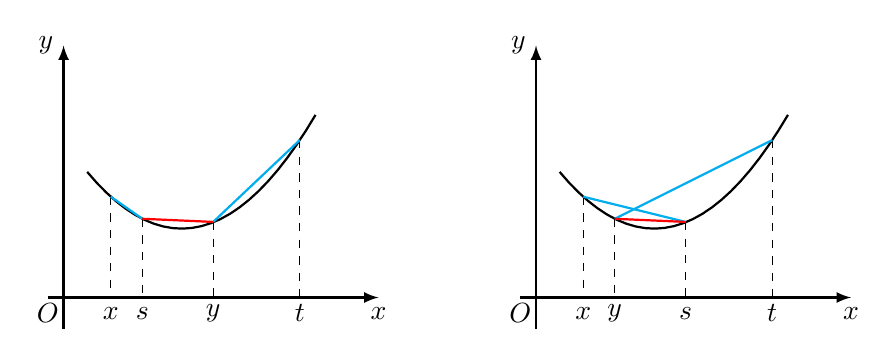
\begin{tikzpicture}[domain=0:4]
\draw[-latex,thick] (-0.2,0) -- (4,0) node[below] {$x$};
\draw[-latex,thick] (0,-0.4) -- (0,3.2) node[left] {$y$};
\node at (-0.2,-0.2){$O$};
\draw[thick,domain=0.3:3.2] plot(\x,0.5*\x*\x-1.5*\x+2);
\draw[dashed](0.6,1.28)--(0.6,0);
\draw[dashed](1,1)--(1,0);
\draw[dashed](1.90,0.96)--(1.90,0);
\draw[dashed](3,2)--(3,0);
\draw[color=cyan,thick](0.6,1.28)--(1,1);
\draw[color=cyan,thick](3,2)--(1.90,0.96);
\draw[color=red,thick](1,1)--(1.9,0.96);
      
 \node at (0.6,-0.2) {$x$};
 \node at (1,-0.2) {$s$};
 \node at (1.9,-0.2) {$y$};
\node at (3,-0.2) {$t$};
  
\draw[-latex,thick] (5.8,0) -- (10,0) node[below] {$x$};
\draw[-latex,thick] (6,-0.4) -- (6,3.2) node[left] {$y$};
\node at (5.8,-0.2){$O$};
\draw[thick,domain=6.3:9.2] plot(\x,0.5*\x*\x-7.5*\x+29);
\draw[dashed](6.6,1.28)--(6.6,0);
\draw[dashed](7,1)--(7,0);
\draw[dashed](7.90,0.96)--(7.90,0);
\draw[dashed](9,2)--(9,0);
\draw[color=cyan,thick](6.6,1.28)--(7.90,0.96);
\draw[color=cyan,thick](7,1)--(9,2);
\draw[color=red,thick](7.90,0.96)--(7,1);
\node at (6.6,-0.2) {$x$};
\node at (7,-0.2) {$y$};
\node at (7.9,-0.2) {$s$};
\node at (9,-0.2) {$t$};      
\end{tikzpicture}
\caption{}
\label{fig:c63}
\end{figure}
\begin{proof}

\end{proof}
\end{quiza}
\begin{quizb}
\woe 设\(\alpha<1\), 且正项级数\(\sum_{i=1}^{\infty}a_n\)收敛, 证明\(\sum_{i=1}^{\infty}M_{\alpha}\left(a_1,a_2,\cdots,a_n\right)\)收敛.
\begin{proof}

\end{proof}
\woe 设凸区域\(\varOmega\)内的凸函数\(f\)在点\(\boldsymbol{x}_0\)的偏导数都存在, 证明\(f\)在点\(\boldsymbol{x}_0\)可微.
\begin{proof}

\end{proof}
\woe 设\(E\in\mathbb{R}^n\)为非空凸闭集, \(\boldsymbol{x}_0\notin E\). 证明存在唯一的\(\boldsymbol{x}\in E\)使得\(|\boldsymbol{x}-\boldsymbol{x}_0|=\inf_{\boldsymbol{y}\in E}|\boldsymbol{y}-\boldsymbol{x}_0|\)(如图). 进一步, 对任何\(\boldsymbol{y}\in E\), \([0,1]\)上的函数\(F(\alpha)=|\boldsymbol{x}+\alpha\left(\boldsymbol{y}-\boldsymbol{x}\right)-\boldsymbol{x}_0|^2\)在点\(0\)取得最小值, 以此证明\(\boldsymbol{x}\)是如下不等式的唯一解:\[\inp{\boldsymbol{x}_0-\boldsymbol{x},\boldsymbol{y}-\boldsymbol{x}}\leqslant 0,\qquad\forall\boldsymbol{y}\in E.\]
\begin{proof}

\end{proof}
\woe 设\(E\subset\mathbb{R}^n\)为非空凸闭集, \(\boldsymbol{x}_0\in\partial E\). 证明存在一列\(E\)外的点列\(\{\boldsymbol{x}_k\}\)收敛于\(\boldsymbol{x}_0\).
\begin{proof}

\end{proof}
\woe 设\(E\subset\mathbb{R}\)为非空凸闭集, \(\boldsymbol{x}_0\in\partial E\). 证明存在非零向量\(\boldsymbol{\mu}\)使得\[\inp{\boldsymbol{\mu},\boldsymbol{x}-\boldsymbol{x}_0}\leqslant 0,\forall\boldsymbol{x}_0\in E,\]平面\(\inp{\boldsymbol{\mu},\boldsymbol{x}-\boldsymbol{x}_0}\)称为\(E\)在点\(\boldsymbol{x}_0\)的支撑面.
\woe 设\(f\)是区域\(\varOmega\in\mathbb{R}^n\)中的凸函数. 证明\(f\)的\textbf{上镜集}\(E=\{(\boldsymbol{x},y)\big|y\geqslant f(\boldsymbol{x}),\boldsymbol{x}\in\varOmega\}\)为凸集. 进一步, 证明\(\overline{E}\)也是凸集.

任取\(\boldsymbol{x}_0\in\varOmega\), 设\(\inp{\boldsymbol{\mu},\boldsymbol{x}-\boldsymbol{x}_0}+\inp{\gamma,y-f\left(\boldsymbol{x}_0\right)}=0\)为\(\overline{E}\)在点\((\boldsymbol{x}_0,f\left(\boldsymbol{x}_0\right))\)处的支撑面. 证明\(\gamma<0\)且\[f\left(\boldsymbol{x}\right)\geqslant f\left(\boldsymbol{x}_0\right)-\frac{1}{\gamma}\boldsymbol{\mu}\cdot\left(\boldsymbol{x}-\boldsymbol{x}_0\right),\qquad\forall\boldsymbol{x}\in\varOmega.\]
\woe 试构造严格凸函数\(f\in C^2(\mathbb{R})\)使得\(\left|f(x)\right|<|x|+1\left(\forall x\in\mathbb{R}\right)\).
\woe 设\(\varphi\)为区间\(I\)上值域为\(I\)的严格单调函数, \(n\geqslant 2\). 对于\(a_1,a_2,\cdots,a_n\), 定义\[F(a_1,a_2,\cdots,a_n)=\varphi^{-1}\left(\frac{1}{n}\sum_{k=1}^{n}\varphi(a_k)\right).\]试对一些具体的\(\varphi\)考察\(F\)的性质.
\woe 设\(f_n(x)=1+\frac{x}{1!}+\frac{x^2}{2!}+\cdots+\frac{x^n}{n!}\), 证明:\begin{quizs}
\item 当\(n\)为偶数时, \(f_n(x)\)在实轴上有正的最小值.
\item 当\(n\)为奇数时, \(f_n(x)\)有且仅有一个实根.
\end{quizs}
\begin{proof}
由\(\ee^x\)的Taylor展开知\[\ee^x=f_n(x)+R_n(x),\quad R_n(x)=\frac{\ee^{\theta x}}{(n+1)!},\quad 0<\theta<1.\]

(1)当\(n\)为偶数时, \(n+1\)为奇数. 由\(\ee^x>0\)知, \(f_n(x)>-R_n(x)\). 当\(x\geqslant 0\)时, \(P_n(x)\geqslant 1>0\), 当\(x<0\)时, 则\[f_n(x)>-R_n(x)=-\frac{\ee^{\theta x}}{(n+1)!}x^{n+1}=\frac{\ee^{\theta x}}{(n+1)!}(-x)^{n+1}>0,\]因此, \(n\)为偶数时, 对任何\(x\), \(f_n(x)>0\), 即\(f_n(x)\)有下界, 则必有下确界, 即为最小值.

(2)当\(n\)为奇数时, \(n-1\)为偶数, 由(1)知\(f_n'(x)=f_{n-1}(x)>0\). \(f_n(x)\)在\(\bbr\)上严格单调递增, 由于\(\lim_{x\rightarrow-\infty}f_n(x)=-\infty,f_n(0)=1>0\), 知\(f_n(x)\)由唯一的实零点.
\end{proof}
\woe 设\(f\)为\(\mathbb{R}\)上实函数, \(E\)为\(f\)的左连续但不连续点的全体. 证明\(E\)至多可列.
\woe 设\(f\)为区间\((a,b)\)上的实函数, 满足\(\forall x\in(a,b),\lim_{y\rightarrow x}f(y)\)存在. 设\(E\)为\(f\)的不连续点全体. 证明\(E\)至多可列.
\woe 设\(a_m>0,a_0,a_1,\cdots,a_{m-1}\in\mathbb{R}\),\[g(x)=a_mx^m+a_{m-1}x^{m-1}+\cdots+a_1x+a_0.\]定义\(G(x)=\left(g(x)\right)^2-g'(x)\). 证明: 若\(g\)有\(m\)个不相同的实零点, 则\begin{quizs}
\item 当\(m\)为正奇数时, \(G\)有且仅有\(m+1\)个实零点.
\item 当\(m\)为正偶数时, \(G\)有且仅有\(m\)个实零点.
\end{quizs}
\begin{proof}
设\(g\)的\(m\)个实零点分别为\(x_1,x_2,\cdots,x_m\),  并且\(x_i<x_{i+1}(i=1,2,\cdots,m-1)\). 于是\[g=a_m(x-x_1)(x-x_2)\cdots(x-x_m),\]易得\(g'(x)=a_m\sum_{k=1}^{m}\prod_{i=1,i\ne k}^{m}(x-x_i)\). 于是\[G(x)=a_m^2\prod_{k=1}^{m}(x-x_k)^2-a_m\sum_{k=1}^{m}\prod_{i=1,i\ne k}^{m}(x-x_i)=a_m^2x^{2m}+P(x),\]其中\(P(x)\)是一次数低于\(2m\)的实系数多项式.

(1)若\(m\)为正奇数, 易见\[G(x_1)<0,G(x_2)>0,G(x_3)<0,\cdots,G(x_m)<0,\]即\((-1)^kG(x_k)>0\). \(G(x)\)连续, 由介值定理知存在\(\xi_k\in(x_k,x_{k+1})(k=1,2,\cdots m-1)\)使得\(G(\xi_k)=0\). 注意到\[G(x)\rightarrow+\infty,\quad x\rightarrow\infty,\]故存在充分大的正数\(A\)满足\(A>x_m\)且\(-A<x_1\)使得\(|x|>A-1\)时\(G(x)> 0\). 于是\(G(A)>0,G(-A)>0\). 从而有\(\xi_0\in(-A,x_1),\xi_m\in(x_m,A)\)使得\(G(\xi_0)=G(\xi_m)=0\). 这便得到了\(G(x)\)的\(m+1\)个实零点. 若除诸\(\xi_k(k=0,1,\cdots m)\)之外, \(G(x)\)还有其他实零点.

(2)若\(m\)为正偶数, 同理可得\[G(x_1)>0,G(x_2)>0,\cdots,G(x_m)>0,\]即\((-1)^{k}G(x_k)<0\). 同理有\(\xi_k\in(x_k,x_{k+1})(k=1,2,\cdots,m-1)\)使得\(G(\xi_k)=0\), 也存在\(A>x_m\)使得\(G(A)>0\), 从而有\(\xi_m\in(x_m,A)\)使得\(G(\xi_m)=0\), 这便得到了\(G(x)\)的\(m\)个实零点. 若除诸\(\xi_k(k=1,2,\cdots,m)\)之外, \(G(x)\)还有其他实零点.
\end{proof}
\woe 对于区间\((a,b)\)内的实函数\(f\), 定义\[F(x)=\varliminf_{y\rightarrow x}\frac{f(y)-f(x)}{y-x},\]这里\(F(x)\)的取值可以是\(\pm\infty\). 依次证明:\begin{quizs}
\item 若\(F(x)>0(\forall x\in(a,b))\), 则\(f\)在\((a,b)\)内严格单调增加.
\item 若\(F(x)\geqslant 0(\forall x\in(a,b))\), 则\(f\)在\((a,b)\)内单调增加.
\end{quizs}
\woe 计算\(\inf_{x\in\left(0,\pi/2\right)}\frac{\tan x-x}{x-\sin x}\).

提示: 求使得以下不等式成立的\(\alpha\):\[\tan x+\alpha\sin x\geqslant (1+\alpha)x,\forall x\in\left(0,\frac{\pi}{2}\right).\]
\begin{solution}
\(\alpha=2.\)
\end{solution}
\woe 设\(f\)在\((a,b)\)内连续, 且对任何\(x\in(a,b)\),\[F(x)=\lim_{h\rightarrow 0}\frac{f(x+h)+f(x-h)-2f(x)}{h^2}\]存在. 证明: \(f\)在\((a,b)\)内凸当且仅当\(F\geqslant 0\).
\woe 设\(f\)在\((a,b)\)内连续. 定义\[F(x)=\varliminf_{h\rightarrow 0}\frac{f(x+h)+f(x-h)-2f(x)}{h^2}.\]证明或证伪: \(f\)在\((a,b)\)内凸当且仅当\(F\geqslant 0\), 这里\(F\)取值也有可能为\(+\infty\).
\woe 试在上述练习基础上, 进一步考察各种"广义"导数, "广义"两阶导数(包括左导数右导数等)与函数单调性, 凹凸性之间的关系.
\end{quizb}
\section{微分Darboux定理与比较定理}
\precis{微分不等式,常微分方程比较定理,偏微分方程比较定理}
\begin{theorem}{}{C64}
设\(y\)在\([a,b]\)上二阶可导, \(g\)为\([a,b]\)上的非负函数, \(f\)为\(\mathbb{R}\)上的连续函数, 满足\(y(a)\leqslant 0,y(b)\leqslant 0\),\begin{gather*}
y''(x)=f(y(x))+g(x),\qquad\forall x\in[a,b],\\
yf(y)\geqslant 0,\qquad\forall y\in\mathbb{R}.
\end{gather*}则\(y(x)\leqslant 0,(\forall x\in[a,b])\).
\end{theorem}
\begin{quiza}
\woe 设\(f\)是\((a,+\infty)\)中的实函数, \(f(a^+)\)与\(f(+\infty)\)存在且相等. 证明: 若\(f\)有三阶导数, 则存在\(\xi\in(a,+\infty)\)使得\(f'''(\xi)=0\).
\woe 设实函数\(f\)是\(\left[a,+\infty\right)\)上有界的可微函数, \(|f'|\)单调. 证明:\(\lim_{x\rightarrow+\infty}xf'(x)=0.\)
\begin{proof}
由Darboux定理可知\(|f'|\)的单调性蕴涵\(f'\)的保号性. 不妨设\(f'\)非负, 此时\(f'\)必然单调减少. 否则\(f'\)单调增加, 且有\(x_2>x_1\geqslant a\)使得\(f'(x_2)>f'(x_1)\geqslant 0\). 由中值定理, 当\(x>x_2\)时,\[f(x)-f(x_2)=f'\left(x_2+\theta (x-x_2)\right)(x-x_2)\geqslant f'(x_2)(x-x_2),\]其中\(\theta\in(0,1)\)与\(x\)有关. 从而\(\lim_{x\rightarrow+\infty}f(x)=+\infty\). 这与题设矛盾. 于是\(f'\)非负且单调减少. 由中值定理,\[2\left(f(x)-f\left(\frac{x}{2}\right)\right)=f'\left(\frac{x}{2}+\alpha\frac{x}{2}\right)x\geqslant f'(x)x\geqslant 0,\]其中\(\alpha\in(0,1)\)为与\(x\)有关的一个数. 由于\(f\)有界, 而由\(f'\)非负知\(f\)单调增加, 所以\(\lim_{x\rightarrow+\infty}f(x)\)存在. 于是由夹逼准则得\(\lim_{x\rightarrow+\infty}xf'(x)=0.\)
\end{proof}
\woe 设一元实函数\(f\)在\([a,b]\)上连续, 在\((a,b)\)内可导, \(ab>0\). 证明\(\xi\in (a,b)\)使得\(\frac{af(b)-bf(a)}{a-b}=f(\xi)-\xi f'(\xi).\)
\woe 设一元实函数\(f\)在\([a,b]\)可微, \(f'(a)=f'(b)\). 证明: 存在\(\xi\in (a,b)\)使得\(f'(\xi)=\frac{f(\xi)-f(a)}{\xi-a}.\)
\begin{proof}
不妨设\(a=0,f(a)=0\), 若结论不真, 则成立\[f'(x)>\frac{f(x)}{x},\quad x\in (0,b)\]或\[f'(x)<\frac{f(x)}{x},\quad x\in (0,b).\]
不妨设前者成立, 于是\[\left(\frac{f(x)}{x}\right)'=\frac{xf'(x)-f(x)}{x^2}>0,\]取\(0<\alpha<\beta<b\), 则对任意\(x\in (0,b),y\in (\beta,b)\)有\[\frac{f(x)}{x}<\frac{f(\alpha)}{\alpha}<\frac{f(\beta)}{\beta}<\frac{f(y)}{y}<f'(y),\]于是令\(x\rightarrow 0^+,y\rightarrow b^-\)有\(f'(a)\ne f'(b)\)矛盾.
\end{proof}
\woe 设一元实函数\(f\)在\([0,1]\)上连续, 在\((0,1)\)内可导, \(f(0)=0,f(1)=1\). 证明存在两两不同的\(\alpha,\beta,\gamma\in (0,1)\)使得\[\frac{1}{f'(\alpha)}+\frac{1}{f'(\beta)}+\frac{1}{f'(\gamma)}=3.\]
\begin{proof}
由中值定理, \(\exists \alpha\in(0,1)\)使得\(f'(\alpha)=\frac{f(1)-f(0)}{1-0}=1\).
\begin{asparaenum}[\textbf{情形}I]
\item \(f(\alpha)=\alpha\), 则由中值定理, 存在\(\beta\in(0,\alpha),\gamma\in(\alpha,1)\)使得\[f'(\beta)=\frac{f(\alpha)-f(0)}{\alpha-0}=1,\quad f'(\gamma)=\frac{f(1)-f(\alpha)}{1-\alpha}=1.\]此时结论成立.
\item \(f(\alpha)<\alpha\), 则存在\(\eta\in(0,\alpha),\zeta\in(\alpha,1)\)使得\[f'(\eta)=\frac{f(\alpha)-f(0)}{\alpha-0}<1,\quad f'(\zeta)=\frac{f(1)-f(\alpha)}{1-\alpha}>1.\]于是有\(\varepsilon>0\)使得\[f'(\eta)<\frac{1}{1+\varepsilon}<1<\frac{1}{1-\varepsilon}<f'(\zeta).\]由Darboux定理, \(\exists\beta\in(\eta,\alpha)\)以及\(\gamma\in(\alpha,\zeta)\)使得\[f'(\beta)=\frac{1}{1+\varepsilon},\quad f'(\gamma)=\frac{1}{1-\varepsilon}.\]立即得到此时结论也成立.
\item \(f(\alpha)>\alpha\). 类似情形II可证.\qedhere
\end{asparaenum}
\end{proof}
\woe 设\(\mu>0\), 一元实函数\(f\)在\([a,b]\)上连续, 在\((a,b)\)内可导, \(c\in(a,b)\)且\(f'(c)=0\). 求证: 存在\(\xi\in(a,b)\)使得\(f'(\xi)=\mu\left(f(\xi)-f(a)\right)\).
\begin{proof}
由于\[\left(f(x)-\int_{a}^{x}\mu\left(f(t)-f(a)\right)\dd t\right)'=f'(x)-\mu\left(f(x)-f(a)\right),\]因此由Darboux定理, \(f'-\mu\left(f-f(a)\right)\)在\((a,b)\)内满足介值性. 

于是若结论不成立, 则\(f'-\mu\left(f-f(a)\right)\)在\((a,b)\)内恒正或恒负. 不妨设
\begin{equation}\label{jiashe666}
f'(x)-\mu\left(f(x)-f(a)\right)>0,\quad x\in(a,b),\tag{$\circledast$}
\end{equation}
则\[\left(\ee^{-\mu x}\left(f(x)-f(a)\right)\right)'=\ee^{-\mu x}\left(f'(x)-\mu\left(f(x)-f(a)\right)\right)>0,\quad\forall x\in(a,b).\]所以\[\ee^{-\mu x}\left(f(x)-f(a)\right)>\ee^{-\mu a}\left(f(a)-f(a)\right)=0,\quad\forall x\in(a,b],\]即\[f(x)-f(a)>0,\quad\forall x\in(a,b].\]于是, 由式\eqref{jiashe666}有\[f'(c)>\mu\left(f(c)-f(a)\right)>0,\]与\(f'(c)=0\)矛盾, 证毕.
\end{proof}
\woe 设实函数\(f\)在\([0,1]\)上连续, 在\((0,1)\)内二阶可导, \(f(0)=0,f\left(\frac{1}{2}\right)=\frac{\pi}{6},f(1)=\frac{\pi}{2}\). 证明: 存在\(\xi\in(0,1)\)使得\(f''(\xi)=\frac{\xi}{1-\xi^2}f'(\xi)\).
\begin{proof}
令\(F(x)=\sqrt{1-x^2}f(x),G(x)=f(x)-\arcsin x\), 于是\(G(0)=G\left(\frac{1}{2}\right)=G(1)=0\), 由Rolle定理知\(\exists \xi_1\in\left(0,\frac{1}{2}\right),\xi_2\in\left(\frac{1}{2},1\right)\)使得\[G'(\xi_1)=G'(\xi_2)=0,\]此时\(f'(\xi_1)=\frac{1}{\sqrt{1-\xi_1^2}},f'(\xi)=\frac{1}{\sqrt{1-\xi_2^2}}\)有\[F(\xi_1)=f'(\xi_1)\sqrt{1-\xi_1^2}=1=f'(\xi_2)\sqrt{1-\xi_2^2}=F'(\xi_2),\]故\(\exists \xi\in\left(\xi_1,\xi_2\right)\)使得\(F'(\xi)=0\), 即得结论.
\end{proof}
%\tcbline
%\begin{proof}
%令\(G(x)=f(x)-\arcsin x\), 则\(G(0)=G\left(\frac{1}{2}\right)=G(1)=0\),由Rolle定理知\(\exists \xi_1\in\left(0,\frac{1}{2}\right),\xi_2\in\left(\frac{1}{2},1\right)\)使得\[G'(\xi_1)=G'(\xi_2)=0,\]又有\(\xi\in\left(\xi_1,\xi_2\right)\)使得\[G''(\xi)=f''(\xi)-\frac{\xi}{1-\xi^2}\cdot\frac{1}{\sqrt{1-\xi^2}}=0\]
%\end{proof}

\woe 设\(f.g\)均为有界闭区间上的单调增加函数, \(F=f-g\)在\([a,b]\)上有介值性. 证明\(F\in C[a,b]\).
\woe 设\(f\)在\(\mathbb{R}^n\)的单位开球\(B_1(\boldsymbol{0})\)内二阶连续可微, 在\(\overline{B_1(\boldsymbol{0})}\)上连续, 满足\(\sum_{k=1}^{n}\frac{\partial^2f(\boldsymbol{x})}{\partial x_k^2}=1-2|\boldsymbol{x}|^2\). 且对任何\(\boldsymbol{x}\in\partial B_1(\boldsymbol{0}),f(\boldsymbol{x})=0\). 试求\(f\)并说明理由.
\end{quiza}
\begin{quizb}
\woe 试根据定理\reff{Th:C64}的证明写出比定理\reff{Th:C64}更一般的结果.
\woe 给定区间\(I\), 试选取其上的一元实函数(记为\(g\)), 求其一阶, 二阶导数, 找出其满足某个二阶微分方程(记为(E)), 选取该函数或导函数在某三点的值, 构造三组数据. 考察一个二阶可导的函数\(f\), 若\(f\)对应的三组数据与\(g\)对应的一样, 是否存在某个\(\xi\in I\)使得\(f\)在\(\xi\)满足方程(E)?

例如, 选取\(I=[0,1],g(x)=x^3\), 则\(g'(x)=3x^2,g''(x)=6x\). 我们有\(3g(x)g''(x)=2\left(g'(x)\right)^2,g''(x)g'(x)=18g(x),g(0)=0,g(1)=1,g'(1)=3\). 我们可以提出以下问题: 

设\(f\)在\([0,1]\)可导, 在\((0,1)\)上两阶可导, \(f(0)=0,f(1)=1,f'(1)=3\). 问是否一定存在\(\xi,\eta\in(0,1)\)使得\(2f(\xi)f''(\xi)=2\left(f'(\xi)\right)^2,f''(\eta)f'(\eta)=18f(\eta)?\)
\woe 设实函数\(f\)在\([a,b]\)上连续, 在\((a,b)\)内有二阶导数, 满足\(f(a)=f(b)=0\). 证明: 若在\((a,b)\)内成立以下条件之一, 则在\([a,b]\)上恒有\(f(x)\leqslant 0\):\begin{quizcs}
\item \(f''(x)-f(x)\geqslant 0\);
\item \(f''(x)-4f'(x)+4f(x)\geqslant 0\);
\item \(f''(x)+4f'(x)+f(x)\geqslant 0\).
\end{quizcs}
\begin{proof}
我们证明这样一个结果: 设\(f\)为题设函数, 若\(f\)满足条件\(f''+\alpha f'+\beta f\geqslant 0\), 其中实数\(\alpha,\beta\)满足\(\alpha^2-4\beta\geqslant 0\), 则\(f\)在\([a,b]\)上恒有\(f\leqslant 0\).

我们有\[f''(x)+\alpha f'(x)+\beta f(x)=\left((\DD-\delta)^2-\gamma\right)f(x)=\ee^{-\delta x}(\DD^2-\gamma)\left(\ee^{\delta x}f(x)\right),\]其中\(\delta=\frac{\alpha}{2},\gamma=\frac{\alpha^2-4\beta}{4}\geqslant 0\).

置\(F(x)=\ee^{\delta x}f(x),\) 设\(F\)在\([a,b]\)上连续, 在\((a,b)\)内有二阶导数, 且\[F''(x)-\gamma F(x)=\ee^{\delta x}\left(f''(x)+\alpha f'(x)+\beta f(x)\right)\geqslant 0,\quad \forall x\in(a,b).\]
\begin{asparaenum}[(i)]
\item 若\(\gamma=0\), 则\(F\)为凸函数, 立即得到\(F(x)\leqslant 0(\forall x\in[a,b])\), 即\(f(x)\leqslant 0(\forall x\in[a,b])\).
\item 若\(\gamma>0\). 此时, 若结论不真, 则有\(\xi\in(a,b)\)使得\(F(\xi)=\max_{x\in[a,b]}F(x)>0\). 我们有\(F''(x)<0\). 另一方面, 由假设条件, \(F''(\xi)\geqslant\gamma F(\xi)>0\). 矛盾, 因此必有\(f(x)\leqslant 0(\forall x\in[a,b])\).
\end{asparaenum}

利用上述结论即证.
\end{proof}
\woe 设\(f\)为\(\mathbb{R}\)上的非负连续可微函数, 满足: \(\forall x\in\mathbb{R}\), 成立\(f'(x)\geqslant 6+f(x)-f^2(x)\). 证明: \(\forall x\in\mathbb{R}\), 成立\(f(x)\geqslant 3\).
\begin{proof}
考虑函数\(g(x)=\frac{f(x)-3}{f(x)+2}\ee^{5x}\), 则\[g'(x)=\frac{5\ee^{5x}\left(f'(x)-6-f(x)+f^2(x)\right)}{\left(f(x)+2\right)^2}\geqslant 0,\]从而\(g(x)\)单调增, 如果存在\(x_0\)使得\(f(x_0)<3\), 则\(g(x_0)<0\)并且\(\forall x<x_0\)都有\(g(x)\leqslant g(x_0)<0\), 从而\(0\leqslant f(x)<3\), 于是有\[-\frac{3}{2}\leqslant\frac{f(x)-3}{f(x)+2}<0,\quad x<x_0,\]这表示\(-\frac{3}{2}\ee^{5x}<g(x)<0\), 令\(x\rightarrow-\infty\)得\(g(x)\rightarrow 0\), 这与任何\(x<x_0\), \(g(x)\leqslant g(x_0)<0\)矛盾.
\end{proof}
\woe 设\(f\)为\(\mathbb{R}\)上的非负连续可微函数, 满足: \(\forall x\in\mathbb{R}\), 成立\(f'(x)\leqslant 6+f(x)-f^2(x)\). 证明: \(\forall x\in\mathbb{R}\), 成立\(f(x)\leqslant 3\).
\begin{proof}
考虑函数\(g(x)=\frac{3-f(x)}{f(x)+2}\ee^{5x}\), 则\[g'(x)=\frac{5\ee^{5x}\left(6+f(x)-f^2(x)-f'(x)\right)}{\left(f(x)+2\right)^2}\geqslant 0,\]从而\(g(x)\)单调增, 如果存在\(x_0\)使得\(f(x_0)>3\), 则\(g(x_0)<0\)并且\(\forall x<x_0\)都有\(g(x)\leqslant g(x_0)<0\), 从而\(f(x)>3\), 于是有\[-1\leqslant\frac{3-f(x)}{f(x)+2}<0,\quad x<x_0,\]这表示\(-\ee^{5x}<g(x)<0\), 令\(x\rightarrow-\infty\)得\(g(x)\rightarrow 0\), 这与任何\(x<x_0\), \(g(x)<g(x_0)<0\)矛盾.
\end{proof}
\woe 设\(f\)在\([a,b]\)上可导, \(g\)在\([a,b]\)上连续. 证明\(F=f'g\)在\([a,b]\)上有介值性质.
\begin{proof}
不失一般性, 只要证明\(F[a,b]\)为区间或单点集. 进一步, 不妨设\(F(a)<\eta<F(b)\), 我们只需要证明存在\(\xi\in(a,b)\)使得\(F(\xi)=\eta\).
\begin{asparaenum}[\bfseries 情形 I]
\item \(\eta=0\). 此时\(f'(a)f'(b)g(a)g(b)<0\). 从而\[f'(a)f'(b)<0\quad\text{或}\quad g(a)g(b)<0.\]若前者成立, 则由微分Darboux定理, 存在\(\xi\in(a,b)\)使得\(f'(\xi)=0\). 若后者成立, 则由连续函数的介值定理, 存在\(\xi\in(a,b)\)使得\(g(\xi)=0\). 无论哪种情形, 都有\(f'(\xi)g(\xi)=\eta\).
\item \(\eta>0\). 此时不妨设\(g(b)>0\).
\begin{compactenum}[(i)]
\item \(g\)在\([a,b]\)上恒正. 则\[f'(a)-\frac{\eta}{g(a)}<0<f'(b)-\frac{\eta}{g(b)},\]而由于函数\(f'-\frac{\eta}{g}\)具有介值性, 因此存在\(\xi\in(a,b)\)使得\(f'(\xi)-\frac{\eta}{g(\xi)}=0\), 即\(f'(\xi)g(\xi)=\eta\).
\item \(g\)在\([a,b]\)上不恒正. 则\(g\)在\([a,b]\)上有最大零点\(s\in[a,b)\). 由微分Darboux定理, 有\((s,b)\)中趋于\(s\)的点列\(\{x_n\}\), 使得\(\lim_{n\rightarrow+\infty}f'(x_n)=f'(s)\). 从而\(\lim_{n\rightarrow+\infty}f'(x_n)g(x_n)=0\). 于是有\(k\geqslant 1\)使得\(f'(x_k)g(x_k)<\eta\). 由于\(g\)在\([x_k,b]\)上恒正, 由(i)可得结论.
\end{compactenum}
\item  \(\eta<0\). 与情形II同理可证.\qedhere
\end{asparaenum}
\end{proof}
\end{quizb}
\section{Taylor多项式与插值多项式}
\precis{Taylor多项式,带Peano型余项的Taylor公式,Maclaurin展开式,Taylor展开式的唯一性,带Lagrange型余项的Taylor公式,Lagrange型插值多项式,线性方程组解的线性可加性,Runge现象,插值多项式的误差估计,插值多项式,插值函数,函数拟合,广义中值定理}
\begin{quiza}
\woe 设\(n\geqslant 2, \delta>0\), 实函数\(f\)在\((x_0-\delta,x+\delta)\)内有定义, 且满足\[f(x)=\sum_{k=0}^{n}a_k(x-x_0)^k+o\left((x-x_0)^n\right),\qquad x\rightarrow x_0.\]
\begin{quizcs}
\item 函数\(f\)在点\(x_0\)是否连续?
\item  若\(f\)在点\(x_0\)连续, \(f\)在点\(x_0\)是否可导?
\item  若\(f\)在点\(x_0\)可导, \(f\)在点\(x_0\)是否二阶可导?
\end{quizcs}
\begin{solution}

\end{solution}
\woe 对于例6.5.4, 记\(k=\frac{6\left(f'(a)+f'(b)\right)}{(b-a)^2}-\frac{12(f(b)-f(a))}{(b-a)^3}\). 尝试通过微分不等式\(f'''>k\)推出矛盾.
\woe 对于例6.5.6, 记\(k=\frac{480\left(f'(a)+4'\left(\frac{a+b}{2}\right)+f'(b)\right)}{(b-a)^4}-\frac{2880\left(f(b)-f(a)\right)}{(b-a)^5}\). 尝试通过微分不等式\(f^{(5)}>k\)推出矛盾.
\woe 设\(f\)在\([0,1]\)上连续, 在\((0,1)\)内可导, 证明存在\(\xi\in(0,1)\)使得\[f'(\xi)=\frac{f(1)+2f\left(\dfrac{1}{2}\right)-3f(0)}{2}\].
\begin{proof}
注意到\[\frac{f(1)+2f\left(\dfrac{1}{2}\right)-3f(0)}{2}=\frac{1}{2}\left(\frac{f(1)-f(0)}{1-0}+\frac{f\left(\dfrac{1}{2}\right)-f(0)}{1/2-0}\right)=\frac{f'(\xi)+f'(\xi_2)}{2},\]其中\(\xi_1\in(0,1),\xi_2\in\left(0,\frac{1}{2}\right),\)并且有\[f'(\xi_1)\wedge f'(\xi_2)\leqslant\frac{f'(\xi_1)+f'(\xi_2)}{2}\leqslant f'(\xi_1)\vee f'(\xi_2),\]由微分Darboux定理可知有\(\xi\)介于\(\xi_1\)与\(\xi_2\)之间满足\(f'(\xi)=\frac{f'(\xi_1)+f'(\xi_2)}{2}\). 从而结论成立.
\end{proof}
\woe 设\(f\)在\([-\sqrt{3},\sqrt{3}]\)上连续, 在\((-\sqrt{3},\sqrt{3})\)上五阶可导. 证明存在\(\xi \in (-\sqrt{3},\sqrt{3})\)使得\[f^{(5)}=5\sqrt{3}\left(f(\sqrt{3})-f(\sqrt{-3})\right)-15\left(f'(-1)+f'(1)\right).\]
\begin{proof}
我们建立更一般的结果. 设\(\alpha>1,f\)在\([-\alpha,\alpha]\)上连续, 在\(\left(-\alpha,\alpha\right)\)内五阶可导, 考虑满足下列条件的五次多项式\(P\):\[\begin{cases}
P(-\alpha)=f(-\alpha),P(-1)=f(-1),P'(-1)=f'(-1),\\
P(1)=f(1),P'(1)=f'(1),P(\alpha)=f(\alpha).
\end{cases}\]则\(P\)由下式唯一确定:\[\left|\begin{matrix}
P(x)&1&x&x^2&x^3&x^4&x^5\\
f(-\alpha)&1&-\alpha&\alpha^2&-\alpha^3&\alpha^4&-\alpha^5\\
f(-1)&1&-1&1&-1&1&-1\\
f(1)&1&1&1&1&1&1\\
f(\alpha)&1&\alpha&\alpha^2&\alpha^3&\alpha^4&\alpha^5\\
f'(-1)&0&1&-2&3&-4&5\\
f'(1)&0&1&2&3&4&5\\
\end{matrix}\right|=0.\]求得\[P^{(5)}=\frac{60\left(f(\alpha)-f(-\alpha)\right)}{\alpha(\alpha^2-1)^2}+\frac{(\alpha^2-3)\left(f(1)-f(-1)\right)}{\left(a^2-1\right)^2}-\frac{30\left(f'(1)+f'(-1)\right)}{\alpha^2-1}.\]考虑\(F=f-P\), 则\(F\)在\([-\alpha,\alpha]\)上连续, 在\((-\alpha,\alpha)\)内五阶可导, 且\[F(-\alpha)=F(\alpha)=F(-1)=F(1)=F'(-1)=F'(1)=0.\]从而存在\(\xi\in(-\alpha,\alpha)\)使得\(F^{(5)(\xi)}=0,\) 即\[f^{5}(\xi)=\frac{60\left(f(\alpha)-f(-\alpha)\right)}{\alpha(\alpha^2-1)^2}+\frac{(\alpha^2-3)\left(f(1)-f(-1)\right)}{\left(a^2-1\right)^2}-\frac{30\left(f'(1)+f'(-1)\right)}{\alpha^2-1}.\]令\(\alpha=\sqrt{3}\), 即得待证明之式.
\end{proof}
\woe 设实函数\(f\)在点\(x_0\)有直到\(n+1\)阶的导数,\[f(x_0+h)=f(x_0)+hf'(x_0)+\frac{h^2}{2!}f''(x_0)+\cdots+\frac{h^n}{n!}f^{(n)}(x_0+\theta_hh),\]其中\(\theta_h\in (0,1)\)与\(h\)的选取有关. \(f^{(n+1)}(x_0)\ne 0.\) 证明: \(\lim_{h\rightarrow 0}\theta_h=\frac{1}{n+1}.\)

进一步, 若\(f^{(n+2)}(x_0)\)存在, 试计算\(\lim_{h\rightarrow 0}\frac{\theta_h-\displaystyle\frac{1}{n+1}}{h}.\)
\begin{proof}
由带Peano余项的Taylor公式:\[f(x_0+h)=f(x_0)+hf'(x_0)+\cdots+\frac{h^n}{n!}f^{(n)}(x_0)+\frac{h^{n+1}}{(n+1)!}f^{(n+1)}(x_0)+o(h^{n+1}),\]于是有\[\frac{h^n}{n!}f^{(n)}(x_0+\theta_hh)=\frac{h^n}{n!}f^{(n)}(x_0)+\frac{h^{n+1}}{(n+1)!}f^{(n+1)}(x_0)+o(h^{n+1}),\]即有\[\theta_h\frac{f^{(n)}(x_0+\theta_hh)-f^{(n)}(x_0)}{\theta_hh}=\frac{1}{n+1}f^{(n+1)}(x_0)+o(h),\]由此易见\(\lim_{h\rightarrow 0}\theta_h=\frac{1}{n+1}.\)

进一步, 由所给条件\[f(x_0+h)=f(x_0)+\cdots+\frac{h^n}{n!}f^{(n)}(x_0)+\frac{h^{n+1}}{(n+1)!}f^{(n+1)}(x_0)+\frac{h^{n+2}}{(n+2)!}f^{(n+2)}(x_0)+o(h^{n+2}),\]于是有\[\frac{h^n}{n!}f^{(n)}(x_0+\theta_hh)=\frac{h^n}{n!}f^{(n)}(x_0)+\frac{h^{n+1}}{(n+1)!}f^{(n+1)}(x_0)+\frac{h^{n+2}}{(n+2)!}f^{(n+2)}(x_0)+o(h^{n+2}),\]即\[f^{(n)}(x_0+\theta_hh)=f^{(n)}(x_0)+\frac{h}{(n+1)}f^{(n+1)}(x_0)+\frac{h^2}{(n+1)(n+2)}f^{(n+2)}(x_0)+o(h^{2}),\]上式两侧减去\(\theta_hhf^{(n+1)}(x_0)\), 得到\[\theta^2_h\frac{f^{(n)}(x+\theta_hh)-f^{(n)}(x_0)-\theta_hhf^{(n+1)}(x_0)}{\theta_h^2h^2}=\frac{\displaystyle\frac{1}{n+1}-\theta_h}{h}f^{(n+1)}(x_0)+\frac{1}{(n+1)(n+2)}f^{(n+2)}(x_0).\]
值得一提的是对于\(f\)有这样的现象\[\lim_{t\rightarrow 0}\frac{f^{(n)}(x_0+t)-f^{(n)}(x_0)-tf^{(n+1)}(x_0)}{h^2}\xlongequal{\text{L'H\^{o}pital}}\frac{1}{2}f^{(n+2)}(x_0).\]
结合上方两式得到\[\frac{\theta_h-\displaystyle\frac{1}{n+1}}{h}\rightarrow\left(\frac{1}{(n+1)(n+2)}-\frac{1}{2(n+1)^2}\right)\frac{f^{(n+2)}(x_0)}{f^{(n+1)}(x_0)},\qquad h\rightarrow 0.\qedhere\]
\end{proof}

\woe 设\(a<c<b\). 试确定常数\(\alpha,\beta,\gamma\), 使得对任何在\([a,b]\)内连续, 在\((a,b)\)内二阶可导的实函数\(f\), 总有\(\xi\in(a,b)\)使得\(f''(\xi)=\alpha f(a)+\beta f(c)+\gamma f(b).\)
\begin{solution}
	
\end{solution}
\woe 设\(a<c<b\). 试确定常数\(\alpha,\beta,\gamma,\delta\), 使得对任何在\([a,b]\)内连续, 在点\(a\)两阶可导, 在\((a,b)\)内三阶可导的实函数\(f\), 总有\(\xi\in(a,b)\)使得\(f'''(\xi)=\alpha f(a)+\beta f(c)+\gamma f(b)+\delta f''(a)\).
\end{quiza}
\begin{quizb}
\woe 对于\(\alpha\in (1,2)\), 尝试构造在\([-\alpha,\alpha]\)上的三阶连续可微的函数\(F\)使得\(F(-\alpha)=F(\alpha)=F'(-1)=F'(1)=0\), 且在\([-\alpha,\alpha]\)上成立\(F'''>0.\)
\begin{solution}

\end{solution}
\woe 设\(a_n\ne -1(n\geqslant 1)\), \(\lim_{n\rightarrow+\infty}a_n=0\), 试在级数\(\sum_{n=1}^{\infty}a_n\)与\(\sum_{n=1}^{\infty}a_n^2\)(绝对)收敛与否的各种情形下, 讨论无穷乘积\(\prod_{n=1}^{\infty}(1+a_n)\)的收敛性(含绝对收敛性).
\begin{solution}

\end{solution}
\woe 证明方程\(x^{2n}-2x^{2n-1}+3x^{2n-2}-\cdots-2nx+(2n+1)=0\)无实根.
\begin{proof}
设\(S(x)=x^{2n}-2x^{2n-1}+3x^{2n-2}-\cdots-2nx+(2n+1)\), 显然\(S(-1)\ne 0\), 注意到\[xS(x)=x^{2n+1}-2x^{2n}+3x^{2n-1}-\cdots-2nx^2+(2n+1)x,\]于是\[S(x)+xS(x)=x-x^2+x^3-\cdots-x^{2n}+x^{2n+1}+(2n+1)=\frac{x\left(1+x^{2n+1}\right)}{1+x}+(2n+1),\]于是\(S(x)=\frac{x(1+x^{2n+1})+(1+x)(2n+1)}{(1+x)^2}\), 即证\(f(x):=x(1+x^{2n+1})+(1+x)(2n+1)\)无除\(x=-1\)外的实根. 由\(f'(x)=0\)可知\(x=-1\)是\(f(x)\)的唯一极小值点, 并且\(f(-1)=0\), 从而结论得证.
\end{proof}
\woe 设\(f(x)\)在\(\mathbb{R}\)上无限次可微, \(f\left(\frac{1}{n}\right)=\frac{n^2}{n^2+1}(\forall n\geqslant1)\), 问以上条件可否确定\(f^{(k)}(0)(\forall k\geqslant 0)\)?
\begin{solution}

\end{solution}
\woe 设\(-\infty<x_1<x_2<\cdots<x_n<+\infty(n\geqslant 2)\), \(P_k(k=1,2,\cdots,n)\)为满足\(P_k(x_j)=\begin{cases}
1,\quad&j=k,\\0,&j\ne k
\end{cases}\)的\(n-1\)次插值多项式. 证明: \(\forall x\in[x_k,x_{k+1}]\), 成立\(P_k(x)+P_{k+1}(x)\geqslant 1(1\leqslant k\leqslant n-1)\).
\begin{proof}
	
\end{proof}
\end{quizb}
\section{Taylor展开式的计算及应用}
\precis{Taylor展开式计算的直接方法和间接方法,利用Taylor展开式计算反函数的高阶导数,利用Taylor展开式计算隐函数的高阶导数,Landau不等式,Taylor展开式在组合问题上的应用}
\begin{quiza}
\woe 计算函数\(f(x)=\left(\frac{1}{7+\cos x}\right)^{1/3}\)的带Peano型余项的三阶Maclaurin展开式.
\begin{solution}

\end{solution}
\woe 将\(\sqrt[3]{1+\sin^3x}\)在点0附近展开到\(x^9\).
\begin{solution}

\end{solution}
\woe 设函数\(f\)在\(x=1\)处有三阶导数, 并满足\(f'(x)=f\left(f(x)\right)\)以及\(f(1)=1.\) 试求\(f\)在\(x=1\)处的带Peano余项的三阶Taylor公式.
\begin{solution}
\(\left(f(x)=1+(x-1)+\frac{1}{2}(x-1)^2+\frac{1}{3}(x-1)^3+o((x-1)^4).\right)\)
\end{solution}
\woe 设定义在点\(0\)附近的光滑函数\(y=y(x)\)满足\(y(0)=0\)以及\(x=\tan y-2y\). 计算\(y(x)\)在\(x=0\)处的带Peano型余项的五阶Taylor公式.
\begin{solution}
\(\left(y=-x-\frac{1}{3}x^3-\frac{2}{27}x^5+o(x^5).\right)\)
\end{solution}
\woe 设光滑函数\(y=y(x)\)满足\(x=\sqrt{y-\ln(1+y)}\mathrm{sgn}(y)\). 试求\(y(x)\)的带Peano型余项的二阶Maclaurin展开式.
\begin{solution}

\end{solution}
\woe 设函数\(y=y(x)\)在\(x=1\)处有五阶导数, \(y(0)=0\), 其反函数\(x=x(y)\)满足: \(x=1+y+3y^2-4y^3+o(y^5)(y\rightarrow 0)\). 试求\(y(x)\)的带Peano型余项的五阶Maclaurin展开式.
\begin{solution}

\end{solution}
\woe 设函数\(y=y(x)\)在\(x=1\)处有三阶导数, \(y(1)=0\), 其反函数\(x=x(y)\)满足:\(x=1+y+3y^2-4y^3+o(y^3)(y\rightarrow 0)\). 试求\(y(x)\)在\(x=1\)处的带Peano型余项的三阶Taylor展开式.
\begin{solution}

\end{solution}
\woe 设实数\(a,A,B\)满足\(\lim_{x\rightarrow\infty}\left[A\left(\cos\frac{1}{x}+a\sin\frac{1}{x^2}+2\cos\frac{1}{x^3}+\sin\frac{1}{x^4}\right)\right]^{x^4}=B\). 试求\(a,A,B\).
\begin{solution}
置\(t=\frac{1}{x}\), 那么原极限即为\[\lim_{t\rightarrow 0}\left[A\left(\cos t+a\sin t^2+2\cos t^3+\sin t^4\right)\right]^{1/t^4},\]该极限存在, 必有\(\lim_{t\rightarrow 0}A\left(\cos t+a\sin t^2+2\cos t^3+\sin t^4\right)=3A=1\), 于是\(A=\frac{1}{3}.\) 另一方面, 我们有\[\cos t+a\sin t^2+2\cos t^3+\sin t^4=3+\left(a-\frac{1}{2}\right)t^2+\frac{25}{24}t^4+o(t^4),\]于是
\[\begin{split}
&\lim_{t\rightarrow 0}\left[A\left(\cos t+a\sin t^2+2\cos t^3+\sin t^4\right)\right]^{1/t^4}\\=&\lim_{t\rightarrow 0}\exp\left(\frac{\ln \left[A\left(\cos t+a\sin t^2+2\cos t^3+\sin t^4\right)\right]}{t^4}\right)\\=&\lim_{t\rightarrow 0}\exp\left(\frac{\displaystyle\frac{1}{3}\left(a-\frac{1}{2}\right)t^2+\frac{1}{3}\cdot\frac{25}{24}t^4+o(t^4)}{t^4}\right)=\exp\left(\frac{25}{72}\right).
\end{split}\]
由此推得\(a=\frac{1}{2},B=\ee^{25/72}.\)
\end{solution}
\woe 设\(f\)在原点有二阶导数, 且\(\lim_{x\rightarrow 0}\left(\frac{\sin 3x}{x^3}+\frac{f(x)}{x^2}\right)=0\). 试求:\begin{quizs}
\item \(f(0),f'(0),f''(0)\);
\item \(\lim_{x\rightarrow 0}\frac{f(x)+3}{x^2}\).
\end{quizs}
\begin{solution}
由假设,\[\frac{\sin3x}{x^3}+\frac{f(x)}{x^2}=o(1),\quad x\rightarrow 0.\]所以\[f(x)=-\frac{\sin 3x}{x}+o(x^2)=-3+\frac{9}{2}x^2+o(x^2),\qquad x\rightarrow 0.\]另外由\(f(x)\)的Taylor展开式\[f(x)=f(0)+f'(0)x+\frac{1}{2}f''(x)x^2+o(x^2),\quad x\rightarrow 0\]的唯一性得到\[f(0)=-3,\quad f(0)=0,\quad f''(0)=9.\]
于是又有\[\lim_{x\rightarrow 0}\frac{f(x)+3}{x^2}=\lim_{x\rightarrow 0}\frac{9x^2/2+o(x^2)}{x^2}=\frac{9}{2}.\qedhere\]
\end{solution}
\woe 设\(n\geqslant 1\), 一元实函数\(f\)在\(\mathbb{R}\)上有\(n+1\)阶导数, 且\(M_0,M_{n+1}<+\infty\), 其中\(M_m=\sup_{x\in\mathbb{R}}|f^{(m)}(x)|(m=0,1,\cdots,n+1)\). 证明: 对于\(1\leqslant m\leqslant n\), 存在与\(f\)无关的常数\(C_m>0\)使得\(M_m<C_mM_0^{1-m/(n+1)}M_{n+1}^{m/(n+1)}\).
\begin{proof}
\(\forall x\in\bbr,h>0\), 存在\(\xi_1,\xi_2,\cdots,\xi_n\)使得\[f(x+mh)=f(x)+\sum_{k=1}^{n}\frac{m^kh^kf^{(k)}(x)}{k!}+\frac{m^{n+1}h^{n+1}f^{(n+1)}(\xi_m)}{(n+1)!},\quad m=1,2,\cdots,n,\]把上式看成\(hf'(x),h^2f''(x),\cdots,h^nf^{(n)}(x)\)的线性方程组, 且方程组的系数矩阵与\(h,f\)无关,  则易见存在与\(f\)和\(h\)无关的常数\(C_1,C_2,\cdots,C_n\)使得\[M_mh^m\leqslant\frac{1}{2}C_m\left(M_0+M_{n+1}h^{n+1}\right),\quad m=1,2,\cdots,n,\]由此利用\(h>0\)的任意性, 取\(h=\left(M_0/M_{n+1}\right)^{1/(n+1)}\), 得到\(M_m<C_mM_0^{1-m/(n+1)}M_{n+1}^{m/(n+1)}\).
\end{proof}
\woe 设\(f\)是\(\left[0,+\infty\right)\)上的有界函数, 有三阶导数, 且\(\lim_{x\rightarrow+\infty}f'''(x)=\alpha\), 其中\(\alpha\in\mathbb{R}\). 证明: \(\lim_{x\rightarrow+\infty}f''(x)=0.\)
\begin{proof}
	由题设, \(\forall\varepsilon>0,\,\exists X\)使得\(x_1,x_2>X\)时有\[\left|f'''(x_1)-f'''(x_2)\right|<\frac{6\varepsilon}{h^3},\]其中\(h\)是给定的正数. 设\(x>X+h\)由Taylor公式\[\begin{split}
		f(x+h)&=f(x)+f(x)h+\frac{f''(x)}{2}h^2+\frac{f'''(\xi_1)}{6}h^3,\quad \xi_1\in(x,x+h),\\
		f(x-h)&=f(x)-f(x)h+\frac{f''(x)}{2}h^2-\frac{f'''(\xi_2)}{6}h^3,\quad \xi_2\in(x-h,x),
	\end{split}\]设\(M\)是\(|f(x)|\)的一个上界, 即有\[\begin{split}
	|f''(x)|&=\left|\frac{f(x+h)+f(x-h)-2f(x)-h^3\left(f'''(\xi_1)-f'''(\xi_2)\right)/6}{h^2}\right|\\&\leqslant\frac{4M+\varepsilon}{h^2}\rightarrow 0,\quad h\rightarrow+\infty.\qedhere
	\end{split}\]
\end{proof}
\woe 设有界数列\(\{a_n\}\)满足\(\lim_{n\rightarrow+\infty}\left(a_{n+2}-2a_{n+1}+a_n\right)=0\), 问是否有\(\lim_{n\rightarrow+\infty}\left(a_{n+1}-a_n\right)=0?\)
\begin{solution}
	结论是成立的. 由题设\(\forall\varepsilon>0\), 存在\(N'\in\bbn\)使得\(n>N'\)时有\[\left|a_{n+2}-2a_{n+1}+a_{n}\right|<\frac{\varepsilon}{2N},\]其中\(N\in\bbn_+\), 设\[
	a_{n+k+1}-2a_{n+k}+a_{n+k-1}=\varepsilon_{k},\quad k=1,2,\cdots N,\]其中\(|\varepsilon_{k}|<\frac{\varepsilon}{2N}\), 我们记上述方程组为\(\boldsymbol{A}\boldsymbol{a}=\boldsymbol{\varepsilon}\), 也即\[\left(\begin{matrix}
	-2&	1&	&	&	\\
	 1&	-2&	1&	&	\\
	  &	\ddots&	\ddots&	\ddots&	\\
		&&1&-2&1\\
		&&&1&	-2\\
	\end{matrix}\right)_{N\times N}\left(\begin{matrix}
	a_{n+1}\\
	a_{n+2}\\
	\vdots\\
	a_{n+N-1}\\
	a_{n+N}
	\end{matrix}\right)=\left(\begin{matrix}
	\varepsilon_1-a_n\\
	\varepsilon_2\\
	\vdots\\
	\varepsilon_{N-1}\\
	\varepsilon_{N}-a_{n+N+1}
	\end{matrix}\right),\]立即可以得到\(\boldsymbol{a}=\boldsymbol{A}^{-1}\boldsymbol{\varepsilon}\), 可以算的\[\boldsymbol{A}^{-1}=\left(\begin{matrix}\vspace{0.4em}
	-\frac{N}{N+1}&-\frac{N-1}{N+1}&\cdots&-\frac{1}{N+1}\\\vspace{0.4em}
	-\frac{N-1}{N+1}&-\frac{2(N-1)}{N+1}&\cdots&-\frac{2}{N+1}\\\vspace{0.4em}
	-\frac{N-2}{N+1}&-\frac{2(N-2)}{N+1}&\cdots&-\frac{3}{N+1}\\\vspace{0.4em}
	\vdots&\vdots&&\vdots\\\vspace{0.4em}
	-\frac{2}{N+1}&\frac{4}{N+1}&\cdots&-\frac{N-1}{N+1}\\\vspace{0.4em}
	-\frac{1}{N+1}&-\frac{2}{N+1}&\cdots&-\frac{N}{N+1}
	\end{matrix}\right)_{N\times N},\]实际上我们只关心\(\boldsymbol{A}^{-1}\)的前两行, 这样得到\[\begin{split}
	a_{n+1}&=-\left(\frac{N}{N+1}\left(\varepsilon_1-a_n\right)+\frac{N-1}{N+1}\varepsilon_2+\frac{N-2}{N+1}\varepsilon_3+\cdots+\frac{\varepsilon_N-a_{n+N+1}}{N+1}\right),\\
	a_{n+2}&=-\left(\frac{N-1}{N+1}\left(\varepsilon_1-a_n\right)+\frac{2(N-1)}{N+1}\varepsilon_2+\frac{2(N-2)}{N+1}\varepsilon_3+\cdots+\frac{2(\varepsilon_N-a_{n+N+1})}{N+1}\right),
	\end{split}\]从而
	\[\begin{split}
		|a_{n+2}-a_{n+1}|&=\left|\frac{\varepsilon_1-a_n}{N+1}-\frac{N-1}{N+1}\varepsilon_2-\frac{N-2}{N+1}\varepsilon_3-\cdots-\frac{\varepsilon_N-a_{n+N+1}}{N+1}\right|\\
		&\leqslant\left|\frac{\varepsilon_1}{N+1}\right|+\left|\frac{N-1}{N+1}\varepsilon_1\right|+\left|\frac{N-2}{N+1}\varepsilon_3\right|+\cdots+\left|\frac{\varepsilon_N}{N+1}\right|+\frac{|a_n|+|a_{n+N-1}|}{N+1}\\
		&\leqslant|\varepsilon_1|+|\varepsilon_2|+\cdots+|\varepsilon_N|+\frac{|a_n|+|a_{n+N-1}|}{N+1}\leqslant\frac{\varepsilon}{2}+\frac{2M}{N+1},
	\end{split}\]其中\(M\)为\(\{|a_n|\}\)的一个上界. 对于\(\varepsilon\), 有充分大得\(N\)使得\(\frac{2M}{N+1}<\frac{\varepsilon}{2}\), 即有\(|a_{n+2}-a_{n+1}|<\varepsilon\), 从而结论成立.
\end{solution}
\end{quiza}
\begin{quizb}
\woe 考察如何求\(\sec x\)的Maclaurin展开式.
\begin{solution}
	1
\end{solution}
\woe 考察含参变量的Taylor展开式. 具体的, 设\(m\geqslant 1\), 在区域\(\varOmega\times D\subseteq\mathbb{R}^n\times\mathbb{R}^m\)内, \(n+m\)元实函数\(f(\boldsymbol{x},\boldsymbol{y})\)作为\(\boldsymbol{x}\)的函数, 所有不高于\(m\)阶的偏导数均存在. 记\[r(\boldsymbol{x},\boldsymbol{y})=f(\boldsymbol{x},\boldsymbol{y})-\sum_{k=0}^{m}\sum_{\left|\alpha\right|=k}\frac{1}{\alpha!}\frac{\partial^kf}{\partial\boldsymbol{x}^\alpha}(\boldsymbol{x}_0,\boldsymbol{y})(\boldsymbol{x}-\boldsymbol{x}_0)^\alpha.\]问什么条件下成立\(\lim_{\boldsymbol{x}\rightarrow\boldsymbol{x}_0}\sup_{\boldsymbol{y}\in D}\frac{r(\boldsymbol{x},\boldsymbol{y})}{|\boldsymbol{x}-\boldsymbol{x}_0|^m}=0\)?
\begin{solution}
	
\end{solution}
\woe 对于数列\(\{a_n\}\), 定义该数列的各阶差分如下:\[\begin{split}
\Delta a_n&=a_{n+1}-a_n,\qquad n\geqslant 1,\\
\Delta^{j+1}a_n&=\Delta^{j}a_{n+1}-\Delta^{j}a_n,\qquad n\geqslant1,j\geqslant 1.
\end{split}\]
\begin{quizs}
\item 证明: 存在常数\(C\)使得对任何数列\(\{a_n\}\), 整数\(k\geqslant 2\), 成立\[k\sup_{n\geqslant 1}|\Delta a_n|\leqslant C\left(\sup_{n\geqslant 1}|a_n|+k^2\sup_{n\geqslant 1}|\Delta^2 a_n|\right).\]
\item 证明: 存在常数\(C_1,C_2\)使得对任何数列\(\{a_n\}\), 整数\(k\geqslant 3\), 成立\[k\sup_{n\geqslant 1}|\Delta a_n|\leqslant C_1\left(\sup_{n\geqslant 1}|a_n|+k^3\sup_{n\geqslant 1}|\Delta^3 a_n|\right)\]以及\[k^2\sup_{n\geqslant 1}|\Delta^2 a_n|\leqslant C_2\left(\sup_{n\geqslant 1}|a_n|+k^3\sup_{n\geqslant 1}|\Delta^3 a_n|\right).\]
\item 试考察更高阶差分的结果.
\end{quizs}
\begin{proof}
	(1)对于任何\(k\geqslant 2\), 我们有\[a_{n+k}-a_n=\sum_{\ell=0}^{k-1}\Delta a_{n+\ell}=k\Delta a_n+\sum_{\ell=1}^{k-1}\left(\Delta a_{n+\ell}-\Delta a_n\right)=k\Delta a_n+\sum_{\ell=1}^{k-1}\sum_{m=0}^{\ell-1}\Delta^2a_{n+m},\]因此,\[k\sup_{n\geqslant 1}|\Delta a_n|\leqslant 2\sup_{n\geqslant 1}|a_n|+\frac{k^2}{2}\sup_{n\geqslant 1}|\Delta^2a_n|,\]取\(C\geqslant 2\)即得结论.
	
	(2)对于任何\(k\geqslant 3\), 我们有\[\begin{split}
		a_{n+k}-a_n&=k\Delta a_n+\frac{k(k-1)}{2}\Delta^2a_n+\sum_{\ell=2}^{k-1}\sum_{m=1}^{\ell-1}\sum_{p=0}^{m-1}\Delta^3a_{n+p},\\
		a_{n+2k}-a_n&=2k\Delta a_n+k(2k-1)\Delta^2a_n+\sum_{\ell=2}^{2k-1}\sum_{m=1}^{\ell-1}\sum_{p=0}^{m-1}\Delta^3a_{n+p},
	\end{split}\]于是\[\begin{split}
		\left(\begin{matrix}
			k\Delta a_n\\ k^2\Delta^2a_n
		\end{matrix}\right)&=\left(\begin{matrix}
			1&\frac{k-1}{2k}\\2&2-\frac{1}{k}
		\end{matrix}\right)^{-1}\left(\begin{matrix}
			a_{n+k}-a_n-\sum_{\ell=2}^{k-1}\sum_{m=1}^{\ell-1}\sum_{p=0}^{m-1}\Delta^3a_{n+p}\\
			a_{n+2k}-a_n-\sum_{\ell=2}^{2k-1}\sum_{m=1}^{\ell-1}\sum_{p=0}^{m-1}\Delta^3a_{n+p}
		\end{matrix}\right)\\
		&=\left(\begin{matrix}
			2-\frac{1}{k}&\frac{1-k}{2k}\\
			-2&1
		\end{matrix}\right)\left(\begin{matrix}
			a_{n+k}-a_n-\sum_{\ell=2}^{k-1}\sum_{m=1}^{\ell-1}\sum_{p=0}^{m-1}\Delta^3a_{n+p}\\
			a_{n+2k}-a_n-\sum_{\ell=2}^{2k-1}\sum_{m=1}^{\ell-1}\sum_{p=0}^{m-1}\Delta^3a_{n+p}
		\end{matrix}\right),
	\end{split}\]由此立即得到\[k\sup_{n\geqslant 1}|\Delta a_n|\leqslant\frac{5}{2}\left(2\sup_{n\geqslant 1}|a_n|+\frac{k^3}{6}\sup_{n\geqslant 1}|\Delta^3a_n|\right)\]以及\[k^2\sup_{n\geqslant 1}|\Delta^2a_n|\leqslant 3\left(2\sup_{n\geqslant 1}|a_n|+\frac{k^3}{6}\sup_{n\geqslant 1}|\Delta^3a_n|\right),\]结论得证.
	
	(3)我们猜测对于\(p,q\in\bbn\)且\(p<q\)有常数\(C\)使得\[k^p\sup_{n\geqslant 1}|\Delta^pa_n|\leqslant C\left(\sup_{n\geqslant 1}|a_n|+k^q\sup_{n\geqslant 1}|\Delta^qa_n|\right),\]
	我们以后再来验证结论的正确性.
\end{proof}
\woe 在习题\(\boldsymbol{\mathcal{A}}\)第10题中, 若函数的定义域是有界区间, 是否有类似的结果?
\begin{solution}
	
\end{solution}
\woe 试构造实数列\(\{a_n\}\)使得\(\sum_{n=1}^{\infty}a_n\)收敛而\(\sum_{n=1}^{\infty}\arctan a_n\)发散.
\begin{solution}
	取\(a_n=\frac{\cos(2\pi n/3)}{n^{1/3}}\), 由Dirichlet判别法可知$\sum_{n=1}^{\infty}a_n$收敛. 但\[a_n^3=\frac{\cos^3(2\pi n/3)}{n}=\frac{1}{n}+\frac{3\cos(2\pi n/3)}{n},\]从而\(\sum_{n=1}^{\infty}a_n^3\)发散, 又\(\arctan a_n\sim a_n-\frac{a_n^3}{3}(a_n\rightarrow 0)\), 并且\(\sum_{n=1}^{\infty}a_n^k(k>3)\)收敛, 从而\(\sum_{n=1}^{\infty}\arctan a_n\)发散.
\end{solution}
\woe 设实函数\(f\)在点\(0\)附近有定义, \(f(0)=0,\lim_{x\rightarrow 0}\frac{f(x)}{x}=1\). 若级数\(\sum_{n=1}^{\infty}a_n\)收敛蕴含\(\sum_{n=1}^{\infty}f(a_n)\)收敛, 证明或证伪: 存在\(\delta>0\)使得对任何\(x\in\left(-\delta,\delta\right)\), 有\(f(x)=x\).
\begin{proof}
	
\end{proof}
\woe 设\(x_0>1,x_1>0,x_{n+2}=x_{n+1}+\frac{x_n}{\ln x_n}(n\geqslant 0)\).
\begin{quizs}
\item 计算\(c\equiv\lim_{n\rightarrow+\infty}\frac{\ln^2x_n}{n}\)以及\(\lim_{n\rightarrow+\infty}\frac{\ln^2x_n-cn}{\sqrt{n}}\).
\item 尝试给出比上述结果更精细的结果.
\end{quizs}
\begin{solution}
(1)

(2)
\end{solution}
\woe 仿第7题编写一些习题.
\end{quizb}